\documentclass[headsepline,11pt,bibliography=leveldown]{scrbook}


\usepackage[utf8]{inputenc}
\usepackage[a4paper]{geometry}
\usepackage{amsmath,amsfonts,amsthm,amssymb}
\usepackage[ngerman]{babel}
\usepackage{float}
\usepackage{tikz}
\usepackage{xcolor}
\usepackage{hyperref}
\usepackage{doi}
\usepackage{graphicx}
\usepackage{helvet}

\usepackage{listings}

\definecolor{codegreen}{rgb}{0,0.6,0}
\definecolor{codegray}{rgb}{0.5,0.5,0.5}
\definecolor{codepurple}{rgb}{0.58,0,0.82}
\definecolor{backcolour}{rgb}{0.95,0.95,0.92}

\lstdefinestyle{mystyle}{
    backgroundcolor=\color{backcolour},   
    commentstyle=\color{codegreen},
    keywordstyle=\color{magenta},
    numberstyle=\tiny\color{codegray},
    stringstyle=\color{codepurple},
    basicstyle=\ttfamily\footnotesize,
    breakatwhitespace=false,         
    breaklines=true,                 
    captionpos=b,                    
    keepspaces=true,                 
    numbers=left,                    
    numbersep=5pt,                  
    showspaces=false,                
    showstringspaces=false,
    showtabs=false,                  
    tabsize=2
}

\lstset{style=mystyle}

\usepackage[backend=biber, style=alphabetic]{biblatex}
\addbibresource{Referenzen.bib}

\newtheorem{lem}{Lemma}[section]
\newtheorem{thm}[lem]{Satz}
\newtheorem{df}[lem]{Definition}

\def\R{\mathbb R}
\def\C{\mathbb C}
\def\N{\mathbb N}
\def\P{\mathbb P}
\def\E{\mathbb E}

\DeclareMathOperator{\vol}{vol}

\usepackage{enumitem}
\parindent0pt
\raggedbottom

\newcounter{NewZaehler}
\newcommand{\NewZahl}{\refstepcounter{NewZaehler}4.\theNewZaehler}

\newenvironment{NewSatz}[1]{\par\medskip\textbf{Satz \NewZahl} #1\textbf{:}~~}{\par\medskip}
\newenvironment{NewDefinition}[1]{\par\medskip\textbf{Definition \NewZahl} #1\textbf{:}~~}{\par\medskip}
\newenvironment{NewBeispiel}[1]{\par\medskip\textbf{Beispiel \NewZahl} #1\textbf{:}\\}{\par\medskip}
\newenvironment{NewBemerkung}[1]{\par\medskip\textbf{Bemerkung \NewZahl} #1\textbf{:}\\}{\par\medskip}
\newenvironment{NewBeweis}[1]{\textit{Beweis} #1\textit{:}\\}{\begin{flushright}$\Box$\end{flushright}}

\newcommand{\en}[1]{{\scriptsize(\textit{#1})}}
\newcommand{\kom}[1]{\ignorespaces}
\newcommand{\red}[1]{{\color{red}#1}}
\newcommand{\green}[1]{{\color{green}#1}}
\newcommand{\Cov}{\operatorname{Cov}}
\newcommand{\Do}{\operatorname{do}}
\newcommand{\ACE}{\operatorname{ACE}}
\newcommand{\Pa}{\operatorname{Pa}}
\newcommand{\pa}{\operatorname{pa}}
\newcommand{\Bild}{\operatorname{Im}}
\newcommand{\Poiss}{\operatorname{Poiss}}

\tikzstyle{endo} = [rectangle, draw, fill=white, minimum size=2em]
\tikzstyle{invis} = [draw=none]

\begin{document}
\setcounter{chapter}{3}
\chapter{Interventionen}
Ausgearbeitet von: {\sffamily\bfseries -}\\

\setcounter{section}{-1}
\section{Abstract}
In diesem Abschnitt geht es um die Grundlagen der kausalen Inferenz, also die Frage, wie man aus statistischen Daten kausale Zusammenhänge zwischen Variablen ableiten kann.\\

Zu Beginn werden wir uns nach einer Wiederholung der Werkzeuge, die wir in diesem Abschnitt benötigen werden mit Korrelation und Kausalität beschäftigen. Dann wird das wichtige Konzept der Interventionen vorgestellt und die Anpassungsformel erarbeitet. Diese wird zur Regel vom kausalen Effekt und zur abgeschnittenen Produktregel verallgemeinert.\\

\section{Überblick}
Ziel der \textit{kausalen Inferenz} ist es einer Wirkung mögliche Ursachen zuzuordnen. Dies soll nach Möglichkeit aus statistischen Daten erfolgen. Das Problem ist hierbei, dass statistische Relationen kausale nicht eindeutig einschränken. Dies werden wir später am Kausalprinzip sehen.\\

In diesem Abschnitt werden wir einige Schritte auf der Hierarchie der kausalen Inferenz \en{causal hierarchy} gehen. Diese hat die folgenden drei Stufen \cite[S. 1]{Paper}.
\begin{enumerate}[label=(\roman*)]
\item Assoziation
\item Intervention
\item Kontrafaktisches
\end{enumerate}
\textit{Assoziation} \en{association} beschreibt das bloße erkennen \en{seeing}, dass es einen statistischen Zusammenhang zwischen den beobachtete Variablen gibt. Bei der \textit{Intervention} \en{intervention} werden Änderungen in Variablen durchgeführt \en{doing}. Bei der \textit{Kontrafaktion} \en{counterfactual} werden sich diese Änderungen nur noch vorgestellt \en{imagining}. Dies ist das typische \glqq Was-wäre-wenn\grqq{}-Spiel.

\section{Wiederholung}
In diesem Kapitel werden wir die nötigen Werkzeuge einführen, die wir für diesen Abschnitt benötigen. Diese sind elementar und benötigen nur grundlegende Kenntnisse aus der Maß- und Wahrscheinlichkeitstheorie. Der Einfachheit halber werden wir meist diskrete Zufallsvariablen betrachten.\\

Wir benötigen einige Male den Begriff der bedingten Wahrscheinlichkeit und der bedingte Erwartung. Wir wiederholen daher folgende
\begin{NewDefinition}{(Bedingte Wahrscheinlichkeit  und bedingte Erwartung)\cite[S. 50]{MWT}}
Sei $X$ eine Zufallsvariable mit Wert $x$ und $Y$ ein Zufallsvektor mit Wert $y$. Sei weiter die Wahrscheinlichkeit $\mathbb{P}(Y = y) > 0$. Dann ist die \textit{bedingte Wahrscheinlichkeit} von $X = x$ unter der Bedingung $Y = y$ definiert durch
\[\mathbb{P}(X = x \mid Y = y) := \frac{\mathbb{P}(X = x, Y = y)}{\mathbb{P}(Y = y)}~.\]
Seien $x_1, \dots, x_n$ alle Werte von $X$. Dann ist die \textit{bedingte Erwartung} von $X$ unter der Bedingung $Y = y$ definiert durch
\begin{align*}
\mathbb{E}(X \mid Y = y) &:= \sum_{i=1}^n x_i \cdot \mathbb{P}(X = x_i \mid Y = y)\\
&= \sum_{i=1}^n x_i \frac{\mathbb{P}(X = x_i, Y = y)}{\mathbb{P}(Y = y)}~.
\end{align*}
\end{NewDefinition}

Weiter benötigen wir noch den Begriff der stochastischen Unabhängigkeit.
\begin{NewDefinition}{(Stochastische Unabhängigkeit)\cite[S. 52]{MWT}}
Seien $X$ und $Y$ Zufallsvariablen. $X$ und $Y$ heißen \textit{stochastische unabhängig}, wenn für alle Kombinationen von Werten $x$ von $X$ und $y$ von $Y$ gilt
\[\mathbb{P}(X = x, Y = y) = \mathbb{P}(X = x) \cdot \mathbb{P}(Y = y)~.\]
\end{NewDefinition}

\begin{NewBemerkung}{(Stochastische Unabhängigkeit und bedingte Wahrscheinlichkeit)}
Seien $X$ und $Y$ stochastisch unabhängige Zufallsvariablen. Aus der Definition der bedingten Wahrscheinlichkeit folgt dann
\begin{align*}
\mathbb{P}(X = x \mid Y = y) &= \frac{\mathbb{P}(X = x, Y = y)}{\mathbb{P}(Y = y)}\\
&= \frac{\mathbb{P}(X = x) \cdot \mathbb{P}(Y = y)}{\mathbb{P}(Y = y)}\\
&= \mathbb{P}(X = x)~.
\end{align*}
Man sagt auch, dass die gemeinsame Verteilungen von unabhängigen Zufallsvariablen in das Produkt der Verteilungen zerfällt.
\end{NewBemerkung}

Weiter benötigen wir noch den
\begin{NewSatz}{(Satz der totalen Wahrscheinlichkeit)\cite[S. 51]{MWT}}
Seien $X$ und $Y$ Zufallsvariablen. Sei $x$ ein Wert von $X$ und $y_1, \dots, y_n$ alle Werte von $Y$. Dann gilt folgende Zerlegung
\[\mathbb{P}(X = x) = \sum_{i=1}^n \mathbb{P}(X = x \mid Y = y_i) \cdot \mathbb{P}(Y = y_i)~.\]
\end{NewSatz}

Außerdem ist ein grundlegendes Verständnis von Kausalgraphen \en{causal graph} notwendig. Wie der Name sagt, beschreibt er kausale Zusammenhänge zwischen verschiedene (Zufalls-)Variablen in einem System graphisch. Wir treffen also die folgende
\begin{NewDefinition}{(Kausal- und Korrelationsgraph)\cite[S. 24 f]{Primer}}
Ein \textit{Kausalgraph} \en{SCM} ist ein gerichteter, azyklischer Graph. Die Knoten des Graphen beschreiben die betrachteten Variablen und die Pfeile dazwischen die Richtung des kausalen Zusammenhangs.\\
Ein \textit{Korrelationsgraph} ist ein ungerichteter Graph. Die Knoten des Graphen beschreiben wieder die betrachteten Variablen und die Linien dazwischen die Assoziationen der Variablen.
\end{NewDefinition}

Bei azyklische Graphen kann eine Variable sich nicht selbst beeinflussen. In der Realität ist es aber häufig der Fall. Dafür betrachten wir das folgende
\begin{NewBeispiel}{(Zyklischer Graph)}
Wir wollen des Zusammenhang zwischen Gehalt $G$ und Inflation $I$ betrachten.\\

\begin{minipage}{0.8\linewidth}
Wir erkennen, dass es einen (kausalen) Zusammenhang zwischen Inflation und Gehalt gibt. Bei einer hohen Inflation muss das Gehalt erhöht werden, da man sich sonst nichts mehr kaufen kann.\\
Umgekehrt beeinflusst das Gehalt aber auch die Inflation. Bekommen die Menschen mehr Geld, so wird das Geld immer weniger Wert. Der Kausalgraph ist rechts abgebildet.\\
\end{minipage}
\begin{minipage}{0.2\linewidth}
\begin{center}
\begin{tikzpicture}[->,>=stealth,shorten >=1pt,auto,node distance=1.5cm,semithick]  
  \node[endo] (G)  {$G$};
  \node[endo] (I) [below of=G] {$I$};

  \path (G) edge node {} (I);
  \path (I) edge node {} (G);
\end{tikzpicture}
\end{center}
\end{minipage}
Solche Beispiele wollen wir in diesem Abschnitt ausschließen, da dies bei der Regel vom kausalen Effekt zu Problemen führen würde.
\end{NewBeispiel}

\begin{NewBemerkung}{(Unterschied Kausal- und Korrelationsgraph)}
Bei den Graphen ist es wichtig zu unterscheiden, auf welchem Level der kausal Inferenz man sich befindet. Betrachtet man nur den assoziativen Level, so ist der Graph als Graph über korrelative Zusammenhänge zu betrachten. Diese Zusammenhänge lassen sich aus gemessenen Daten ablesen. Nach Definition sollte der Korrelationsgraph eigentlich keine Pfeilspitzen enthalten. Durch Intuition und Logik wird dieser Graph trotzdem meiste mit Pfeilen versehen.\\
Betrachtet man den Graphen hingegen aus einer intervenierenden Sicht, so geht man davon aus, dass jeder Pfeil im Graphen einem kausalen Zusammenhang entspricht. Wir verwenden als Modell meist den gerichteten Korrelationsgraphen.\\
Der Übergang von dem Korrelationsgraphen zu dem Kausalgraphen ist ein sehr gewagter Schritt. Wir werden später sehen, dass nicht jede Korrelation einen direkten kausalen Zusammenhang impliziert.
\end{NewBemerkung}

Bei den Knoten des Graphen müssen wir zwei Typen unterscheiden.

\begin{NewDefinition}{(Exogene und endogene Variablen)\cite[S. 27 f]{Primer}}
\textit{Exogene Variablen} \en{exogenous variables} sind Variablen, deren Werte außerhalb eines gegebenen Modells bestimmt werden, womit darauf kein Einfluss genommen werden kann. Sie werden als gegeben und unabhängig von allen anderen Variablen angenommen. Bezeichnet werden die Variablen mit $U_X, U_Y, U_Z, \dots$ und ihre Werte mit $u_X, u_Y, u_Z, \dots$.\\
\textit{Endogene Variablen} \en{endogenous variables} sind Variablen, die durch Zustände, die im Modell stattfindet und durch die exogenen Variablen bestimmt werden. Bezeichnet werden die Variablen mit $X, Y, Z, \dots$ und ihre Werte mit $x, y, z, \dots$.\\
Wir setzen voraus, dass wir endogene Variablen also Funktionen von anderen Variablen.
\end{NewDefinition}

\begin{NewBemerkung}{Strukturelles Modelle \cite[S. 27]{Monografie}}
Ein System solcher Gleichungen für die endogenen Variablen wird als \textit{strukturelles Gleichungsmodell} \en{structural equation model} bezeichnet. Ist ein kausaler Graph zugrunde gelegt, so heißt das Modell \textit{strukturelles kausales Modell} \en{structural causal model}.\\
Die exogenen Variablen $U_X, U_Y, U_Z, \dots$ können als Störung interpretiert werden.\\
Wir können die strukturelle Gleichung einer Variablen $X$ schreiben als
\[X := f_X(\Pa(X), U_X)~.\]
Hierbei ist $\Pa(X)$ die Menge der Eltern \en{parents} von $X$. Da wir voraussetzen, dass dieser Zusammenhang gilt, verwenden wir \glqq $:=$\grqq{} und sehen diese Gleichung als eine Festlegung an.\\
Meist sind die strukturellen Gleichungen lineare Funktion. Es lässt sich darüber streiten, inwieweit sich die Realität durch lineare Funktion beschreiben oder approximieren lässt.
\end{NewBemerkung}

In den Graphen sind die endogenen Variablen mit einem Kasten abgebildet und die exogenen ohne.

\begin{NewBeispiel}{(Pflanzenwachstum)}
Zur Einführung dieser neuen Begriffe wollen wir als Beispiel die Größe einer Pflanze $G$ modellieren. Wir verwenden hier einen Kausalgraphen.\\

\begin{minipage}{0.5\linewidth}
Als endogene Variablen modellieren wir das Wasser $W$ und das Licht $L$, dass der Pflanze zur Verfügung steht. Beides wird von dem äußerem Einfluss des Wetters $U_{W, L}$ beeinflusst. Wir können Wasser auch durch Gießen $U_W$ hinzufügen. Andere äußere Einflüsse wie das genetische Material der Pflanze seien mit $U_G$ bezeichnet. Der Kausalgraph ist rechts zu sehen.\\
\end{minipage}
\begin{minipage}{0.5\linewidth}
\begin{center}
\begin{tikzpicture}[->,>=stealth,shorten >=1pt,auto,node distance=1.5cm,semithick]  
  \node (U_X) {$U_G$};
  \node (U_Y) [right of=U_X] {$U_W$};
  \node (U_{Y, Z}) [right of=U_Y] {$U_{W, L}$};
  \node[invis] (H) [below of=U_X] {};
  \node[endo] (Y) [below of=U_Y] {$W$};
  \node[endo] (Z) [below of=U_{Y, Z}] {$L$};
  \node[endo] (X) [below of=H] {$G$};

  \path (U_{Y, Z}) edge node {} (Z);
  \path (U_{Y, Z}) edge node {} (Y);
  \path (U_Y) edge node {} (Y);
  \path (U_X) edge node {} (X);
  \path (Z) edge node {} (X);
  \path (Y) edge node {} (X);
\end{tikzpicture}
\end{center}
\end{minipage}

Wir sehen also, dass die Pflanzengröße $G$ eine Funktion von Wasser $W$, Sonne $L$ und weiteren Einflüssen $U_G$ ist. Wir können also auch schreiben
\[G = f_G(W, L, U_G)~.\]

\begin{minipage}{0.5\linewidth}
\begin{center}
\begin{tikzpicture}[->,>=stealth,shorten >=1pt,auto,node distance=2cm,semithick]  
  \node (U_X) {$U_G$};
  \node[invis] (U_Y) [right of=U_X] {$w$};
  \node (U_{Y, Z}) [right of=U_Y] {$U_{W, L}$};
  \node[invis] (H) [below of=U_X] {};
  \node[endo] (Y) [below of=U_Y] {$W = w$};
  \node[endo] (Z) [below of=U_{Y, Z}] {$L$};
  \node[endo] (X) [below of=H] {$G$};

  \path (U_{Y, Z}) edge node {} (Z);
  \path (U_Y) edge node {} (Y);
  \path (U_X) edge node {} (X);
  \path (Z) edge node {} (X);
  \path (Y) edge node {} (X);
\end{tikzpicture}
\end{center}
\end{minipage}
\begin{minipage}{0.5\linewidth}
Wir können einen Kausalgraphen auch modifizieren \en{graph surgery} \cite[S. 54]{Primer}. In obigem Pflanzenbeispiel können wir beispielsweise eine Apparatur bauen, die dafür sorgt, dass die Pflanze genau die Menge $w$ an Wasser erhält. Man denke an ein lichtdurchlässiges Dach. Durch diese Fixierung haben wir die exogene Variable $U_W$ aus dem Modell entfernt und die Abhängigkeit von $U_{W, L}$ und $W$ aufgehoben. Die Auswirkungen auf den Graphen sind links abgebildet.\\
\end{minipage}
\end{NewBeispiel}

\section{Kausalität und Korrelation}
Wie wir im vorigen Kapitel gesehen haben, scheint der Begriff der Kausalität zentral zu sein. Wir gehen daher einen Schritt zurück und wollen uns fragen, was Kausalität überhaupt ist.

\begin{NewDefinition}{(Kausalität)\cite[S. 26]{Primer}\cite[S. 5]{Paper}}
Seien $X$ und $Y$ Zufallsvariablen. Wir sagen $X$ \textit{verursacht} $Y$ \en{cause}\kom{S. 5}, wenn die Werte von $Y$ in irgendeiner Weise von den Werten von $X$ abhängen.
\end{NewDefinition}

\begin{NewBemerkung}{(Eigenschaften der Kausalität)}
Dies ist der klassische \glqq Ursache-Wirkung\grqq{}-Zusammenhang. Der Kausalgraph einer Ursache $X$ mit Wirkung $Y$ ist denkbar einfach.
\begin{center}
\begin{tikzpicture}[->,>=stealth,shorten >=1pt,auto,node distance=2cm,semithick]  
  \node (X) {$X$};
  \node (Y) [right of=X] {$Y$};

  \path (X) edge node {} (Y);
\end{tikzpicture}
\end{center}
Man sagt auch $X$ und $Y$ sind kausal abhängig. Kausalität ist allgemein keine symmetrische Eigenschaft. Viel mehr gilt das \textit{Kausalprinzip} \cite[S. 3]{Paper}. Seien $X$ und $Y$ statisch abhängig. Dann gilt genau eine der folgenden Aussagen.
\begin{enumerate}[label=(\roman*)]
\item $X$ folgt aus $Y$
\item $Y$ folgt aus $X$
\item Es gibt eine Variable $Z$, sodass $X$ und $Y$ jeweils aus $Z$ folgen
\end{enumerate}
Im letzten Fall werden $X$ und $Y$ unabhängig, wenn auf $Z$ bedingt wird. Wir sehen also, dass Kausale- und stochastische Unabhängigkeit sehr verschiedene Begriffe zu sein scheinen. 
\end{NewBemerkung}

\begin{NewBeispiel}{(Kausale- und Stochastische Abhängigkeit)}
Wir betrachten ein Skat-Deck mit $32$ Karten und ziehen ohne Zurücklegen zwei Stück. Seien $X$ und $Y$ Zufallsvariablen mit
\begin{align*}
X &= \begin{cases}
1 &,\,\text{erste Karte schwarz}\\
0 &,\,\text{sonst}
\end{cases}\\
Y &= \begin{cases}
1 &,\,\text{beide Karten gleiche Farbe}\\
0 &,\,\text{sonst}~.
\end{cases}
\end{align*}
Es gilt dann
\begin{alignat*}{2}
\mathbb{P}(X = 1) &= \frac{16}{32} &&= \frac{1}{2}\\
\mathbb{P}(Y = 1) &= 2 \cdot\frac{16}{32} \cdot \frac{15}{31} &&= \frac{15}{31}\\
\mathbb{P}(X = 1, Y = 1) &= \frac{16}{32} \cdot \frac{15}{31} &&= \frac{15}{62}\\
\mathbb{P}(X = 1) \cdot \mathbb{P}(Y = 1) &= \frac{16}{32} \cdot \frac{15}{31} &&= \frac{15}{62}~.
\end{alignat*}
Also ist $\mathbb{P}(X = 1, Y = 1) = \mathbb{P}(X = 1) \cdot \mathbb{P}(Y = 1)$. Durch analoge Rechnungen erhält man dann das gleiche für die anderen Kombinationen. Somit sind $X$ und $Y$ stochastisch unabhängig.\\
Wir erkennen aber, dass $X$ und $Y$ kausal abhängig sind, da die Farbe der ersten Karte das Ergebnis, dass beide Karten die gleiche Farbe haben mit beeinflusst.\\
Stochastische- und kausale Abhängigkeit sind also unterschiedliche Begriffe.
\end{NewBeispiel}

Nun werden wir anhand eines Beispiels sehen, dass Kausalität allgemein nicht symmetrisch ist.
\begin{NewBeispiel}{(Symmetrie der Kausalität)}
Sei $X$ ein Zufallsvariable mit Wert $1$, wenn es regnet und $0$ sonst. Beschreibe $Y$ nun den Zustand der Straße mit gleichen Werten. Dann führt $X = 1$ sofort zu $Y = 1$, aber umgekehrt $Y = 1$ nicht zu $X = 1$.\\
Regen führt dazu, dass die Straße nass ist. Ist die Straße nass, so muss es umgekehrt nicht unbedingt geregnet haben. Es kann sein, dass jemand sein Auto gewaschen hat und die Straße dadurch nass wurde.\\
Wir erkennen also führt $X$ zu $Y$, so führt allgemein $Y$ nicht zu $X$. Somit ist die Verbindung von Zufallsvariablen im Kausalgraphen durch Pfeile sehr sinnvoll.
\end{NewBeispiel}

Verwandt mit dem Begriff der Kausalität ist der Begriff der Korrelation.
\begin{NewDefinition}{(Korrelation)\cite[S. 56]{MWT}}
Seien $X$ und $Y$ Zufallsvariablen. Wir sagen $X$ und $Y$ sind \textit{korreliert} \en{correlated}\kom{S. 22}, wenn ihre \textit{Kovarianz} nicht verschwindet. Es soll also gelten
\[\Cov(X, Y) = \mathbb{E}(XY) - \mathbb{E}(X) \mathbb{E}(Y) \neq 0~.\]
Man sagt auch $X$ und $Y$ sind \textit{assoziiert}. Es sei erwähnt, dass Assoziation eigentlich ein allgemeinerer Begriff ist, als Korrelation. Für die hier verwendeten Zwecke kann man die Begriffe allerdings als äquivalent ansehen.
\end{NewDefinition}

\begin{NewBemerkung}{(Eigenschaften der Korrelation)}
An der Definition erkennen wir, dass Korrelation symmetrisch ist. Das folgt direkt aus der Kommutativität der reellen Zahlen. Wir erkennen also, dass Korrelation und Kausalität ebenfalls unterschiedliche Begriffe sein müssen.
\end{NewBemerkung}

Dazu betrachten wir folgendes
\begin{NewBeispiel}{(Eisverkauf)\cite[S. 54f]{Primer}}
Sei $E$ eine Zufallsvariable, welche die Anzahl an verkauften Eiskugeln modelliert. Weiter sei $D$ eine Zufallsvariable, welche die Anzahl der aufgetretenen Taschendiebstählen misst. Wir haben die folgenden Daten gemessen.
\begin{center}
\begin{tabular}{| l | c | c | c | c | c | c | c | c | c | c | c |}
\hline
$E$ & $1860$ & $1985$ & $2211$ & $2215$ & $2712$ & $2387$ & $2801$ & $2912$ & $3058$ & $3032$ & $2812$\\
\hline
$D$ & $10$ & $12$ & $11$ & $15$ & $17$ & $18$ & $20$ & $19$ & $22$ & $21$ & $23$\\
\hline
\end{tabular}
\end{center}
\begin{minipage}{0.5\linewidth}
Es scheint demnach so, als würden mehr Eisverkäufe zu einer größeren Anzahl an Verbrechen führen. In der Grafik rechts wurden die Taschendiebstähle gegen die Eisverkäufe abgetragen wurden. Hier wird der Zusammenhang noch deutlicher.\\
Dieser scheinbare kausale Zusammenhang lässt sich logisch jedoch nicht begründen. Ebensowenig Sinn ergibt die Umkehrung, dass mehr Taschendiebstähle zu mehr Eisverkäufen führen.\\
Der Korrelationsgraph ist damit gegeben durch.
\end{minipage}
\begin{minipage}{0.5\linewidth}
\begin{center}
	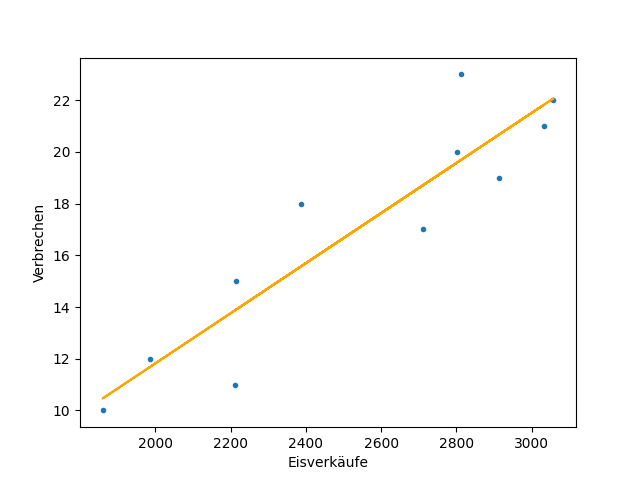
\includegraphics[width=1.1\linewidth]{Eisverkäufe vs Taschendiebstähle.png}
\end{center}
\end{minipage}

\begin{center}
\begin{tikzpicture}[-,>=stealth,shorten >=1pt,auto,node distance=2cm,semithick]
  \node[endo] (Y) {$E$};
  \node[endo] (Z) [right of=Y] {$D$};

  \path (Y) edge node {} (Z);
\end{tikzpicture}
\end{center}

Wir messen nun als dritte Variable noch die Temperatur $T$. Die Daten erweitern sich wie folgt.
\begin{center}
\begin{tabular}{| l | c | c | c | c | c | c | c | c | c | c | c |}
\hline
$T$ & $18$ & $20$ & $21$ & $23$ & $24$ & $25$ & $27$ & $28$ & $29$ & $30$ & $32$\\
\hline
$E$ & $1860$ & $1985$ & $2211$ & $2215$ & $2712$ & $2387$ & $2801$ & $2912$ & $3058$ & $3032$ & $2812$\\
\hline
$D$ & $10$ & $12$ & $11$ & $15$ & $17$ & $18$ & $20$ & $19$ & $22$ & $21$ & $23$\\
\hline
\end{tabular}
\end{center}
Die Grafiken zu Temperatur-Eisverkäufe (links) \kom{Eis-Taschendiebstähle-Temperatur.py} und Temperatur-Taschendiebstähle (rechts) \kom{Eis-Taschendiebstähle-Temperatur.py} zeigen nun ein anderes Bild.\\
\begin{minipage}{0.5\linewidth}
\begin{center}
	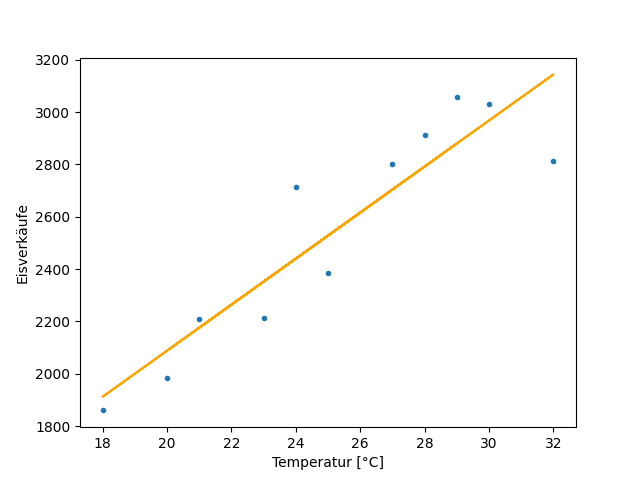
\includegraphics[width=1.1\linewidth]{Temperatur vs Eisverkäufe.png}
\end{center}
\end{minipage}
\begin{minipage}{0.5\linewidth}
\begin{center}
	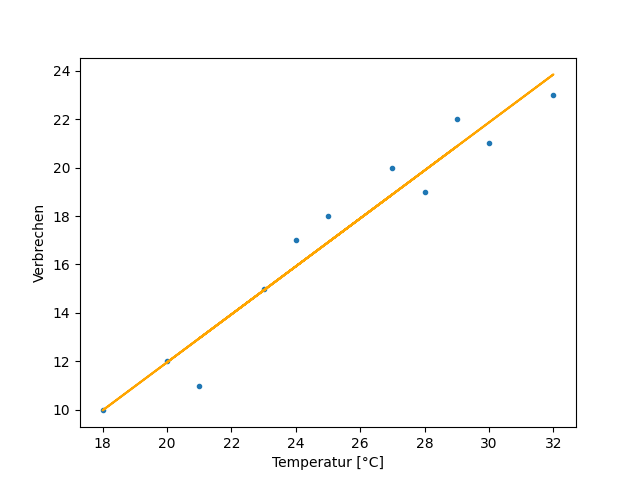
\includegraphics[width=1.1\linewidth]{Temperatur vs Taschendiebstähle.png}
\end{center}
\end{minipage}
\begin{minipage}{0.5\linewidth}
Wir erkenne also, dass der scheinbare Zusammenhang zwischen Eisverkäufen und Verbrechen aus dem jeweiligen kausalen Zusammenhang mit der Temperatur folgt.\\
Dieser lässt sich auch logisch begründen. Bei warmem Wetter essen Passanten mehr Eis und da bei hohen Temperaturen mehr Menschen unterwegs sind, kommt es zu mehr Taschendiebstählen. Der Kausalgraph ist rechts abgebildet.\\
\end{minipage}
\begin{minipage}{0.5\linewidth}
\begin{center}
\begin{tikzpicture}[->,>=stealth,shorten >=1pt,auto,node distance=2cm,semithick]
  \node (U_X) {$U_T$};  
  \node[endo] (X) [below of=U_X] {$T$};
  \node[endo] (Y) [below left of=X] {$E$};
  \node[endo] (Z) [below right of=X] {$D$};
  \node (U_Y) [above of=Y] {$U_E$};
  \node (U_Z) [above of=Z] {$U_D$};

  \path (U_X) edge node {} (X);
  \path (U_Y) edge node {} (Y);
  \path (U_Z) edge node {} (Z);
  \path (X) edge node {} (Y);
  \path (X) edge node {} (Z);
\end{tikzpicture}
\end{center}
\end{minipage}
Dies ist auch ein Beispiel für korrelierte Zufallsvariablen, die nicht kausal zusammenhängen, denn es gilt \kom{Eis-Taschendiebstähle-Temperatur.R}
\[\Cov(E, D) \approx 1771 \neq 0~.\]
Im Bezug auf das Kausalprinzip ist dies also der letzte Fall. Wir haben als dritte Variable die Temperatur $T$ gefunden, die sowohl eine Ursache für die Anzahl der Eisverkäufe $E$ als auch für die Anzahl an Taschendiebstählen $D$ ist.
\end{NewBeispiel}

Wir erkennen an diesem Beispiel auch, dass simple Beobachtungsstudien, die einzelne Parameter messen scheinbar nicht ausreichen, um einen kausalen Zusammenhang zu erkennen oder gar zu beweisen. Wir wollen uns deshalb im nächsten Kapitel mit einer Möglichkeit beschäftigen solche Zusammenhänge besser untersuchen zu können.

\section{Interventionen}
In diesem Kapitel beschäftigen wir uns mit den wichtigsten Konzepten dieses Abschnittes; den Interventionen und dem $\Do$-Calculus.\\

Ziel der Statistik ist es die Effekte von Interventionen vorherzusagen. Sammeln wir beispielsweise Daten über Lungenkrebserkrankungen bei Rauchern, suchen wir Möglichkeiten einzugreifen \en{intervene}, um die Wahrscheinlichkeit an Krebs zu erkranken, zu senken.\\

Wir wollen nun auf die nächste Stufe der Hierarchie der kausalen Inferenz steigen und benötigen daher die folgende
\begin{NewDefinition}{(Intervention)\cite[S. 54]{Primer}\cite[S. 5]{Paper}}
Sei $X$ eine Zufallsvariable und $x$ einer ihrer Werte. Eine \textit{Intervention} ist eine Maßnahme, um den Wert der Zufallsvariable auf $x$ zu fixieren. Dies schreiben wir als $\Do(X = x)$.
\end{NewDefinition}

\begin{NewBemerkung}{(Auswirkungen von Interventionen)\cite[S. 5]{Paper}}
Durch Interventionen werden alle Zusammenhänge von anderen Variablen zu $X$ aufgelöst.\\
Wir nehmen an, dass bei der Intervention $\Do(X = x)$ keine Nebenwirkungen \en{side effects} auftreten. Diese Voraussetzung bezeichnet man auch als \textit{Lokalität} \en{locality}. Insbesondere nehmen wir an, dass die Intervention an $X$ nicht zu einer Änderung im Mechanismus, der die Interaktion der Variablen festlegt, führt.\\
Falls solche Effekte auftreten, müssen wir diese explizit ins Modell aufnehmen.
\end{NewBemerkung}

\begin{NewBeispiel}{(Interventionen)}
Wir zählen einige Beispiele für Intervention auf.
\begin{enumerate}[label=(\roman*)]
\item Im Pflanzenbeispiel haben wir die Wassermenge fixiert.
\item Im Eisverkaufsbeispiel können wir versuchen alle Eisstände zu schließen und somit die Anzahl der verkaufen Eiskugel auf null zu fixieren.
\item Bei einer Untersuchung, ob Rauchen zu Lungenkrebs führt, wird fixiert, ob geraucht wird oder nicht.
\item In einer medizinischen Studie, bei der die Wirksamkeit eines Medikamentes untersucht wird, wird die Gabe des Medikamentes oder eines Placebos fixiert.
\end{enumerate}
\end{NewBeispiel}

\begin{NewBemerkung}{(Unterschied Intervention und Konditionierung)\cite[S. 55]{Primer}\cite[S. 5]{Paper}}
Interventionen finden vor der Messung der Daten statt. Wir gehen also davon aus, dass der gesamte Stichprobenraum \en{population} auf den entsprechenden Wert der Variable fixiert ist.\\
Im Gegensatz dazu findet eine Konditionierung \en{conditioning} erst nach der Messung der Daten statt. Durch bedingte Wahrscheinlichkeiten werden aus den Daten nur die Teile gefiltert, die der Konditionieren entsprechen.
\end{NewBemerkung}

Um den Unterschied näher zu erläutern betrachten wir noch einmal das Eisverkaufsbeispiel.

\begin{NewBeispiel}{(Eisverkauf)}
Die gemessenen Daten haben dieselbe Struktur wie zuvor.
\begin{center}
\begin{tabular}{| l | c | c | c | c | c | c | c | c | c | c | c |}
\hline
$E$ & $1860$ & $1985$ & $2211$ & $2215$ & $2712$ & $2387$ & $2801$ & $2912$ & $3058$ & $3032$ & $2812$\\
\hline
$D$ & $10$ & $12$ & $11$ & $15$ & $17$ & $18$ & $20$ & $19$ & $22$ & $21$ & $23$\\
\hline
\end{tabular}
\end{center}
Wir wollen nun bestimmen, wie viele Taschendiebstähle wir erwarten, wenn höchstens $2500$ Eiskugeln verkauft wurden. Es gilt
\begin{align*}
&\mathbb{E}(D \mid E \leq 2500)\\
&= \frac{10 \cdot \mathbb{P}(D = 10) + 12 \cdot \mathbb{P}(D = 12) + 11 \cdot \mathbb{P}(D = 11) + 15 \cdot \mathbb{P}(D = 15) + 18 \cdot \mathbb{P}(D = 18)}{\mathbb{P}(E < 2500)}~.
\intertext{Da jeder Wert von $D$ nur einmal vorkommt ist die Wahrscheinlichkeit im Nenner je gleichgroß und es gilt}
&= \frac{\frac{1}{11} \cdot (10 + 12 + 11 + 15 + 18)}{\frac{5}{11}}\\
&= \frac{1}{5} \cdot 66 = 13.2~.
\end{align*}
Angenommen wir würden nun intervenieren und die Eisdielen zwingen, dass höchstens $2500$ Eiskugeln am Tag verkauft werden dürfen. Wir führen das Experiment durch und erhalten die folgenden Daten.
\begin{center}
\begin{tabular}{| l | c | c | c | c | c | c | c | c | c | c | c |}
\hline
$E$ & $1860$ & $1985$ & $2211$ & $2215$ & $2500$ & $2387$ & $2500$ & $2500$ & $2500$ & $2500$ & $2500$\\
\hline
$D$ & $10$ & $12$ & $11$ & $15$ & $17$ & $18$ & $20$ & $19$ & $22$ & $21$ & $23$\\
\hline
\end{tabular}
\end{center}
Wir berechnen nun
\begin{align*}
&\mathbb{E}(D \mid \Do(E \leq 2500))\\
&= 10 \cdot \mathbb{P}(D = 10 \mid \Do(E \leq 2500)) + \dots + 23 \cdot \mathbb{P}(D = 23 \mid \Do(E \leq 2500))~.
\intertext{Auch hier kommt jeder Wert von $D$ nur einmal vor und die Wahrscheinlichkeit je gleich groß und es gilt}
&= \frac{1}{11} \cdot (10 + 12 + 11 + 15 + 17 + 18 + 20 + 18 + 22 + 21 + 23)\\
&= \frac{1}{11} \cdot 187 = 17~.
\end{align*}

\begin{minipage}{0.5\linewidth}
Wir haben durch die Intervention dafür gesorgt, dass die Kante, die die Eisverkäufe $E$ mit der Anzahl der Taschendiebstähle $D$ verbinden, verschwinden. Der modifizierte Graph ist rechts abgebildet.\\
Insbesondere haben wir durch die Intervention die exogene Variable $U_E$ aus dem Modell entfernt.\\
Selbst, wenn wir die Wert der Intervention, auf den wir $E$ fixieren ändern, wird diese Änderung nicht an $D$ weitergegeben.
\end{minipage}
\begin{minipage}{0.5\linewidth}
\begin{center}
\begin{tikzpicture}[->,>=stealth,shorten >=1pt,auto,node distance=2cm,semithick]
  \node (U_X) {$U_T$};  
  \node[endo] (X) [below of=U_X] {$T$};
  \node[endo] (Y) [below left of=X] {$E \leq 2500$};
  \node[endo] (Z) [below right of=X] {$D$};
  \node (U_Z) [above of=Z] {$U_D$};
  \node (U_Y) [above of=Y] {$\leq 2500$};

  \path (U_X) edge node {} (X);
  \path (U_Z) edge node {} (Z);
  \path (U_Y) edge node {} (Y);
  \path (X) edge node {} (Z);
\end{tikzpicture}
\end{center}
\end{minipage}
\end{NewBeispiel}

An diesem Beispiel sehen wir also, dass die Intervention bezüglich Variablen zu einem vollständig anderen Muster von Abhängigkeiten führt als die Konditionierung.

\begin{NewBemerkung}{(Notation und Interpretation)\cite[S. 55]{Primer}}
Seien nun $X$ und $Y$ Zufallsvariablen auf einer Bevölkerung und $y$ ein Wert von $Y$.\\
Durch die Konditionierung $\mathbb{P}(X = \cdot \mid Y = y)$ erhalten wir also die Verteilung von $X$ unter der Teilmenge der Individuen \en{individuals} mit $Y = y$.\\
Durch die Intervention $\Do(Y = y)$ nehmen wir an, dass wir eine Bevölkerung mit ausschließlich $Y = y$ hätten. Dann ist $\mathbb{P}(X = \cdot \mid \Do(Y = y))$ die entsprechende Verteilung in dieser Bevölkerung.
\end{NewBemerkung}

Eine Möglichkeit die Intervention zu erreichen ist die \textit{randomisierte kontrollierte Studie} \en{randomized controlled experiments} \cite[S. 53]{Primer}. Dies ist der Goldstandard in Statistik und vor allem Medizin.\\
Wir teilen hier eine Population in zwei Gruppen ein. Innerhalb der Gruppe variieren alle Faktoren, die das Ergebnis beeinflussen, entweder zufällig oder sie werden fixiert. Nach Konstruktion gibt es nur eine Variable, die das Ergebnis beeinflusst. Somit lassen sich signifikante Unterschiede in den Ergebnissen der Gruppen auf diese eine Variable zurückführen. In der Medizin ist der Unterschied zwischen den beiden Gruppen meist, wer die Behandlung erhält und wer ein Placebo.\\
Um Voreingenommenheiten \en{bias} zu vermeiden, sind solche Studien meist \textit{verblindet}. Weiß nur der Teilnehmende nicht, zu welcher Gruppe er gehört, so heißt die Studie \textit{einfachblind}. Weiß der Beobachtende auch nicht, zu welcher Gruppe der Teilnehmende gehört, so heißt sie \textit{doppelblind} und weiß auch der Auswertende nicht, welche Gruppe er betrachtet, so sogar \textit{dreifachblind}.\\

Auch die randomisierte kontrollierte Studie hat einige Probleme.
\begin{enumerate}[label=(\roman*)]
\item Wie kann sicher gestellt werden, dass andere Faktoren effektiv genug kontrolliert werden?
\item Wie viele Teilnehmer werden benötigt, um einen Effekt über statistisches Rauschen hinaus zu \glqq beweisen\grqq{}?
\item Wie wird sicher gestellt, dass Selbstauskünfte wahr sind?
\end{enumerate}
Speziell bei Studien über Medikamente.
\begin{enumerate}[label=(\roman*), resume]
\item Wie werden genetische Faktoren ausgeschlossen?
\item Was passiert, wenn die Probanden ihre Medizin zu spät nehmen oder es (noch nicht entdeckte) Wechselwirkungen mit anderen Substanzen oder Umwelteinflüssen gibt?
\item Wie lassen sich solche Studien realisieren, bei Krankheiten, die nur sehr wenige Menschen betreffen?
\item Wie werden Ergebnisse von Probanden bewertet, die die Studie abbrechen?
\item Ist es überhaupt ethisch vertretbar der einen Hälfte ein Medikament zu verabreichen und der anderen ein Placebo?
\end{enumerate}

\section{Adjustierungsformel}
In diesem Abschnitt werden wir eine Methode kennen lernen, um kausale Zusammenhänge aus reinen Beobachtungsdaten herzuleiten. Wir werden eine Formel finden, um die $\Do$-Wahrscheinlichkeit ohne eine Intervention zu berechnen.\\

Um zu bestimmen, wie stark kausale Effekt einer Variablen auf eine andere ist, benötigen wir noch die folgende
\begin{NewDefinition}{(Durchschnittlicher kausaler Effekt)}
Seien $X$ und $Y$ Variablen und $X$ sogar \textit{binär}, habe also nur die Werte $0$ und $1$. Weiter sei $y$ ein Wert von $Y$. Wir definieren den \textit{durchschnittlichen kausalen Effekt von $X$ auf $Y$} ($\ACE$) \en{average causal effect, causal effect difference} durch
\[\ACE(X \rightarrow Y) := \mathbb{P}(Y = y \mid \Do(X = 1)) - \mathbb{P}(Y = y \mid \Do(X = 0))~.\]
\end{NewDefinition}

Zur Herleitung der Adjustierungsformel betrachten wir das folgende
\begin{NewBeispiel}{(Simpson Paradoxon)\cite[S. 1ff, S. 55 - 58]{Primer}}
Im Simpson Paradoxon wurde beobachtet, dass eine Medikament die Genesungsrate in der Gesamtgruppe zu senken scheint, aber in den nach Geschlechtern getrennten Gruppen jeweils einen positiven Effekt auf die Genesung hat.\\

Sei $M$ die Zufallsvariable die beschreibt, ob das Medikament gegeben wurde oder nicht. Die Werte seinen entsprechend $1$ und $0$. Weiter sei $H$ die Variable, die mit $1$ die Heilung und mit $0$ keine Genesung beschreibt. Außerdem sei $G$ die Zufallsvariable, die das Geschlecht beschreibt. Hierbei stehe $0$ für weiblich und $1$ für männlich. Die Wahrscheinlichkeiten der Genesung waren wie folgt gegeben \cite[S. 2]{Primer}.
\begin{center}
\begin{tabular}{| c | c | c |}
\hline
& $M = 0$ & $M = 1$\\
\hline
$G = 0$ & $55$ von $80$ ($69 \%$) & $192$ von $263$ ($73 \%$)\\
\hline
$G = 1$ & $234$ von $270$ ($87 \%$) & $81$ von $87$ ($93 \%$)\\
\hline
Gesamt & $289$ von $350$ ($83 \%$) & $273$ von $350$ ($78 \%$)\\
\hline
\end{tabular}
\end{center}

\begin{minipage}{0.5\linewidth}
Wir nehmen an, dass das die Gabe des Medikaments $M$ und das Geschlecht $G$ einen Einfluss auf die Genesung $H$ haben. Weiter habe das Geschlecht $G$ eine Auswirkung, mit welcher Wahrscheinlichkeit das Medikament genommen wird. Außerdem werde die Genesung $H$ von einer exogenen Variable $U_H$ beeinflusst. Der Kausalgraph ist rechts abgebildet.\\
Wir sehen, dass die Genesung $H$ eine Funktion von $m$, $g$ und $u_H$ ist. Problematisch ist nur, dass $M$ eine Funktion von $g$ und $u_M$ ist.\\
\end{minipage}
\begin{minipage}{0.5\linewidth}
\begin{center}
\begin{tikzpicture}[->,>=stealth,shorten >=1pt,auto,node distance=2cm,semithick]
  \node (H_eins) {};
  \node (U_Z) [right of=H_eins] {$U_G$};
  \node (H_zwei) [right of=U_Z] {};
  \node (U_X) [below of=H_eins] {$U_M$};
  \node[endo] (Z) [below of=U_Z] {$G$};
  \node (U_Y) [below of=H_zwei] {$U_H$};
  \node[endo] (X) [below of=U_X] {$M$};
  \node[endo] (Y) [below of=U_Y] {$H$};
  
  \path (U_X) edge node {} (X);
  \path (U_Y) edge node {} (Y);
  \path (U_Z) edge node {} (Z);
  \path (Z) edge node {} (X);
  \path (Z) edge node {} (Y);
  \path (X) edge node {} (Y);
\end{tikzpicture}
\end{center}
\end{minipage}

Wir wollen nun wissen, wie gut das Medikament wirkt. Dies ist der Unterschied zwischen der Wahrscheinlichkeit der Genesung, wenn der Medizin gegeben wird und, wenn keine Medizin gegeben wird. Naive würde man
\begin{align*}
\mathbb{P}(H = 1 \mid M = 1) - \mathbb{P}(H = 1 \mid M = 0) &= 78 \% - 83 \%\\
&= - 5 \% < 0
\end{align*}
berechnen und schließen, dass das Medikament nicht wirkt und die Chance für die Heilung sogar verschlechtert. Wie wir im ersten Abschnitt gesehen ist dies aber paradox, da das Medikament für Frauen und Männer die Chance auf Genesung jeweils erhöht. Daher wollen wir nun durchschnittlichen kausalen Effekt
\[\ACE(M \rightarrow H) = \mathbb{P}(H = 1 \mid \Do(M = 1)) - \mathbb{P}(H = 1 \mid \Do(M = 0))\]
bestimmen.\\

\begin{minipage}{0.5\linewidth}
\begin{center}
\begin{tikzpicture}[->,>=stealth,shorten >=1pt,auto,node distance=2cm,semithick]
  \node (H_eins) {};
  \node (U_Z) [right of=H_eins] {$U_G$};
  \node (H_zwei) [right of=U_Z] {};
  \node (U_X) [below of=H_eins] {$m$};
  \node[endo] (Z) [below of=U_Z] {$G$};
  \node (U_Y) [below of=H_zwei] {$U_H$};
  \node[endo] (X) [below of=U_X] {$M = m$};
  \node[endo] (Y) [below of=U_Y] {$H$};
  
  \path (U_X) edge node {} (X);
  \path (U_Y) edge node {} (Y);
  \path (U_Z) edge node {} (Z);
  \path (Z) edge node {} (Y);
  \path (X) edge node {} (Y);
\end{tikzpicture}
\end{center}
\end{minipage}
\begin{minipage}{0.5\linewidth}
Hierfür führen wir eine Intervention durch, um die Abhängigkeit zwischen Geschlecht $G$ und Medikamentengabe $M$ aufzulösen. Das neue Modell ist links abgebildet. Im modifizierten Modell \en{manipulated model} gilt dann
\[\mathbb{P}_m(H = 1 \mid M = m) = \mathbb{P}(H = 1 \mid \Do(M = m))~.\]
Durch $m = 1$ und $m = 0$ können wir nun bestimmen, ob das Medikament genommen wird oder nicht.\\
\end{minipage}

Wir werden sehen, dass nach der Adjustierungsformel gilt
\[\mathbb{P}(H = 1 \mid \Do(M = m)) = \sum_{g \in \{0,1\}} \mathbb{P}(H = 1 \mid M = m, G = g) \cdot \mathbb{P}(G = g)~.\]
Durch einsetzten erhalten wir für die Wahrscheinlichkeit, dass ein Patient sich erholt, wenn wir ihm das Medikament geben
\begin{align*}
\mathbb{P}(H = 1 \mid \Do(M = 1)) &= \mathbb{P}(H = 1 \mid M = 1, G = 0) \mathbb{P}(G = 0) + \mathbb{P}(H = 1 \mid M = 1, G = 1) \mathbb{P}(G = 1)~.
\intertext{Einsetzten der Daten lifert}
&= 73 \% \cdot \frac{263 + 80}{700} + 93 \% \cdot \frac{87 + 270}{700}\\
&= 35.77 \% + 47.43 \% = 83.2 \%~.
\end{align*}
Für die Wahrscheinlichkeit, dass ein Patient sich erholt, wenn wir ihm das Medikament nicht geben, gilt
\begin{align*}
\mathbb{P}(H = 1 \mid \Do(M = 0)) &= \mathbb{P}(D = 1 \mid M = 0, G = 0) \mathbb{P}(G = 0) + \mathbb{P}(H = 1 \mid M = 0, G = 1) \mathbb{P}(G = 1)\\
&= 69 \% \cdot \frac{263 + 80}{700} + 87 \% \cdot \frac{87 + 270}{700}\\
&= 33.81 \% + 44.37 \% = 78.18 \%~.
\end{align*}
Damit erhalten wir also
\begin{align*}
\ACE(M \rightarrow H) &= \mathbb{P}(H = 1 \mid \Do(M = 1)) - \mathbb{P}(H = 1 \mid \Do(M = 0))\\
&= 83.2 \% - 78.18 \%\\
&= 5.02 \% > 0~.
\end{align*}
Somit hat die Einnahme des Medikaments unabhängig vom Geschlecht einen positiven Effekt und das Paradoxon ist aufgelöst.\\
Nach der Adjustierungsformel müssen wir also auf das Geschlecht konditionieren, die Effekte des Medikaments getrennt betrachten und zum Schluss über die Wahrscheinlichkeit des jeweiligen Geschlechts mitteln. Insbesondere dürfen wir die Wahrscheinlichkeiten für eine Erholung mit und ohne Medikament nicht vergleichen.
\end{NewBeispiel}

Nun zum versprochenen
\begin{NewSatz}{(Adjustierungsformel)\cite[S. 57]{Primer} \cite[S. 6]{Paper}}
Seien $X$, $Y$ und $Z$ Zufallsvariablen, sodass $Z$ eine Ursache für $X$ und $Y$ ist. Weiter sei $Y$ noch eine Folge von $X$. Außerdem sei $x$ ein Wert von $X$ und $y$ ein Wert von $Y$. Nach der \textit{Adjustierungsformel} \en{adjustment formula} gilt dann
\[\mathbb{P}(Y = y \mid \Do(X = x)) = \sum_{z \in \Bild(Z)} \mathbb{P}(Y = y \mid X = x, Z = z) \cdot \mathbb{P}(Z = z)~.\]
\end{NewSatz}

\begin{NewBeweis}{\cite[S. 56f]{Primer}}
Es ist links der anfängliche Kausalgraph abgebildet und rechts der modifizierte nach der Intervention.\\

\begin{minipage}{0.5\linewidth}
\begin{center}
\begin{tikzpicture}[->,>=stealth,shorten >=1pt,auto,node distance=2cm,semithick]
  \node (H_eins) {};
  \node (U_Z) [right of=H_eins] {$U_Z$};
  \node (H_zwei) [right of=U_Z] {};
  \node (U_X) [below of=H_eins] {$U_X$};
  \node[endo] (Z) [below of=U_Z] {$Z$};
  \node (U_Y) [below of=H_zwei] {$U_Y$};
  \node[endo] (X) [below of=U_X] {$X$};
  \node[endo] (Y) [below of=U_Y] {$Y$};
  
  \path (U_X) edge node {} (X);
  \path (U_Y) edge node {} (Y);
  \path (U_Z) edge node {} (Z);
  \path (Z) edge node {} (X);
  \path (Z) edge node {} (Y);
  \path (X) edge node {} (Y);
\end{tikzpicture}
\end{center}
\vspace*{0\baselineskip}
\end{minipage}
\begin{minipage}{0.5\linewidth}
\begin{center}
\begin{tikzpicture}[->,>=stealth,shorten >=1pt,auto,node distance=2cm,semithick]
  \node (H_eins) {};
  \node (U_Z) [right of=H_eins] {$U_Z$};
  \node (H_zwei) [right of=U_Z] {};
  \node (U_X) [below of=H_eins] {$x$};
  \node[endo] (Z) [below of=U_Z] {$Z$};
  \node (U_Y) [below of=H_zwei] {$U_Y$};
  \node[endo] (X) [below of=U_X] {$X = x$};
  \node[endo] (Y) [below of=U_Y] {$Y$};
  
  \path (U_X) edge node {} (X);
  \path (U_Y) edge node {} (Y);
  \path (U_Z) edge node {} (Z);
  \path (Z) edge node {} (Y);
  \path (X) edge node {} (Y);
\end{tikzpicture}
\end{center}
\vspace*{0\baselineskip}
\end{minipage}

Nach dieser Modifikation gilt also
\[\mathbb{P}(Y = y \mid \Do(X = x)) = \mathbb{P}_m(Y = y \mid X = x)~.\]
Aufgrund der Lokalität gilt für alle $z \in \Bild(Z)$
\[\mathbb{P}_m(Z = z) = \mathbb{P}(Z = z)~,\]
da der Mechanismus, der $Z$ bestimmt durch die Intervention nicht verändert wurde. Da sich der Prozess, der $Y$ als Funktion von $X$, $Z$ und $U_Y$ bestimmt unter der Intervention nicht ändert, gilt
\[\mathbb{P}_m(Y = y \mid X = x, Z = z) = \mathbb{P}(Y = y \mid X = x, Z = z)~.\]
Durch die Intervention sind $X$ und $Z$ im modifizierten Modell stochastisch unabhängig. Also folgt aus der Bemerkung zur stochastischen Unabhängigkeit
\begin{align*}
\mathbb{P}_m(Z = z \mid X = x) &= \mathbb{P}_m(Z = z)\\
&= \mathbb{P}(Z = z)~,
\end{align*}
wegen der Invarianz der Verteilung von $Z$ unter der Modifikation. Wir führen nun diese Vorüberlegungen zusammen und betrachten
\begin{align*}
\mathbb{P}(Y = y \mid \Do(X = x)) &= \mathbb{P}_m(Y = y \mid X = x))~.
\intertext{Nach dem Satz der total Wahrscheinlichkeit folgt}
&= \sum_{z \in \Bild(Z)} \mathbb{P}_m(Y = y \mid X = x, Z = z) \cdot \mathbb{P}_m(Z = z \mid X = x)~.
\intertext{Da $X$ und $Z$ im modifizierten Modell stochastisch unabhängig sind, folgt}
&= \sum_{z \in \Bild(Z)} \mathbb{P}_m(Y = y \mid X = x, Z = z) \cdot \mathbb{P}_m(Z = z)~.
\intertext{Mit den Invarianzeigenschaften folgt}
&= \sum_{z \in \Bild(Z)} \mathbb{P}(Y = y \mid X = x, Z = z) \cdot \mathbb{P}(Z = z)~.
\end{align*}
Dies ist genau die zu beweisende Gleichung.
\end{NewBeweis}

\begin{NewBemerkung}{\cite[S. 57]{Primer}}
In der Adjustierungsformel sagt man auch, dass man \textit{für $Z$ adjustiert} \en{adjust for $Z$} oder \textit{für $Z$ kontrolliert} \en{controlling for $Z$}.\\
Die Adjustierungsformel ist also eine Gleichung, mit der man die Wahrscheinlichkeit nach einer Intervention aus den bedingten Wahrscheinlichkeiten ohne zu intervenieren berechnen kann.
\end{NewBemerkung}

Wir betrachten nun ein weiteres
\begin{NewBeispiel}{(Blutdruck) \cite[S. 58]{Primer}}
Sei $M$ die Zufallsvariable die beschreibt, ob das Medikament gegeben wurde oder nicht. Die Werte seinen entsprechend $1$ und $0$. Weiter sei $H$ die Variable, die mit $1$ die Genesung und mit $0$ keine Genesung beschreibt. Außerdem sei $B$ die Zufallsvariable, die den Blutdruck nach der Behandlung beschreibt. Hierbei sei $0$ für niedrigen und $1$ für hohen Blutdruck. Die Wahrscheinlichkeiten der Genesung waren wie folgt gegeben \cite[S. 4]{Primer}.
\begin{center}
\begin{tabular}{| c | c | c |}
\hline
& $M = 0$ & $M = 1$\\
\hline
$B = 0$ & $81$ von $87$ ($93 \%$) & $234$ von $270$ ($87 \%$)\\
\hline
$B = 1$ & $192$ von $263$ ($73 \%$) & $55$ von $80$ ($69 \%$)\\
\hline
Gesamt & $273$ von $350$ ($78 \%$) & $289$ von $350$ ($83 \%$)\\
\hline
\end{tabular}
\end{center}
\begin{minipage}{0.5\linewidth}
Wir gehen davon aus, dass die Genesung $H$ sowohl von der Gabe des Medikaments $M$ als auch von dem Blutdruck $B$ beeinflusst wird. Weiter nehmen wir an, dass der Blutdruck vom Medikament beeinflusst wird. Der Kausalgraph ist rechts abgebildet.\\
Wir erkennen einen ähnlichen Kausalgraph wie im Simpson Paradoxon. Hier ist der Pfeil zwischen $M$ und $B$ umgekehrt.\\
Wir wollen wieder testen, ob das Medikament positive Auswirkungen auf die Genesung hat und somit den durchschnittlichen kausalen Effekt $\ACE$ berechnen.\\
\end{minipage}
\begin{minipage}{0.5\linewidth}
\begin{center}
\begin{tikzpicture}[->,>=stealth,shorten >=1pt,auto,node distance=2cm,semithick]
  \node (H_eins) {};
  \node (U_Z) [right of=H_eins] {$U_B$};
  \node (H_zwei) [right of=U_Z] {};
  \node (U_X) [below of=H_eins] {$U_M$};
  \node[endo] (Z) [below of=U_Z] {$B$};
  \node (U_Y) [below of=H_zwei] {$U_H$};
  \node[endo] (X) [below of=U_X] {$M$};
  \node[endo] (Y) [below of=U_Y] {$H$};
  
  \path (U_X) edge node {} (X);
  \path (U_Y) edge node {} (Y);
  \path (U_Z) edge node {} (Z);
  \path (X) edge node {} (Z);
  \path (Z) edge node {} (Y);
  \path (X) edge node {} (Y);
\end{tikzpicture}
\end{center}
\end{minipage}

Wir wollen intervenieren und alle Pfeile, die $M$ beeinflussen, verschwinden lassen. Da $M$ bis auf $U_M$ keine Eltern hat, ist keine Modifikation des Graphen notwendig. Das Experiment war also ausreichend randomisiert. In diesem Fall gilt mit der Adjustierungsformel
\begin{align*}
\mathbb{P}(H = h \mid \Do(M = m)) &= \sum_{b \in \Bild(B)} \mathbb{P}(H = h \mid M = m, B = b) \cdot \mathbb{P}(B = b)~.
\intertext{Da $H$ gegeben $M$ im ursprünglichen Modell schon von $B$ unabhängig waren, gilt}
&= \sum_{b \in \Bild(B)} \mathbb{P}(H = h \mid M = m) \cdot \mathbb{P}(B = b)\\
&= \mathbb{P}(H = h \mid M = m) \sum_{b \in \Bild(B)} \mathbb{P}(B =b)~.
\intertext{Da $\mathbb{P}_B$ ein Wahrscheinlichkeitsmaß ist, vereinfacht sich dies zu}
&= \mathbb{P}(H = h \mid M = m)~.
\end{align*}
Dies kann interpretiert werden als Adjustierung bezüglich der leeren Menge.
\end{NewBeispiel}

\section{Die Regel vom kausalen Effekt}
Im vorigen Abschnitt haben wir gesehen, dass wir bei einer Intervention auf Eltern von $X$ konditionieren müssen, da wir durch die Intervention genau diese Einflüsse neutralisieren.\\
Wir wollen nun die Adjustiertungsformel weiter verallgemeinern. Sei dazu $\Pa(X)$ der Zufallsvektor der Eltern von $X$. Es darf jetzt insbesondere $\left| \Pa(X) \right| > 1$ sein. Dann gilt
\begin{NewSatz}{(Die Regel vom kausalen Effekt) \cite[S. 59]{Primer}}
Sei ein Kausalgraph gegeben und $\Pa(X)$ der Zufallsvektor der Eltern von $X$, sowie $Y$ eine weiter Zufallsvariable. Dann gilt für den kausalen Effekt von $X$ auf $Y$
\[\mathbb{P}(Y = y \mid \Do(X = x)) = \sum_{z \in \Bild(\Pa(X))} \mathbb{P}(Y = y \mid X = x, \Pa(X) = z) \cdot \mathbb{P}(\Pa(X) = z)~.\]
Hierbei seien $y$ und $x$ Werte von $Y$ respektive $X$ und $z$ ein mögliche Kombination von Werten des Vektors $\Pa(X)$.
\end{NewSatz}

\begin{NewBeweis}{}
Sei $\Pa(X) = (Z_1, \dots, Z_n)^\top$ mit $n \in \mathbb{N}$. Dann gilt ähnlich zum Beweis der Adjustierungsformel für den anfänglichen und modifizierten Kausalgraph.\\

\begin{minipage}{0.5\linewidth}
\begin{center}
\begin{tikzpicture}[->,>=stealth,shorten >=1pt,auto,node distance=1.5cm,semithick]
  \node[endo] (X) {$X$};
  \node (H) [below of=X] {};
  \node[endo] (Z_eins) [right of=H] {$Z_1$};
  \node (Punkte) [right of=Z_eins] {$\cdots$};
  \node[endo] (Z_n) [right of=Punkte] {$Z_n$};
  \node[endo] (Y) [below of=H] {$Y$};
  \node (U_X) [above of=X] {$U_X$};
  \node (U_Z_eins) [right of=U_X] {$U_{Z_1}$};
  \node (U_Punkte) [right of=U_Z_eins] {$\cdots$};
  \node (U_Z_n) [right of=U_Punkte] {$U_{Z_n}$};
  \node (U_Y) [below of=Z_n] {$U_Y$};
  
  \path (X) edge node {} (Y);
  \path (Z_eins) edge node {} (Y);
  \path (Z_n) edge node {} (Y);
  \path (U_X) edge node {} (X);
  \path (U_Y) edge node {} (Y);
  \path (U_Z_eins) edge node {} (Z_eins);
  \path (U_Z_n) edge node {} (Z_n);
  \path (Z_eins) edge node {} (X);
  \path (Z_n) edge node {} (X);
\end{tikzpicture}
\end{center}
\vspace*{0\baselineskip}
\end{minipage}
\begin{minipage}{0.5\linewidth}
\begin{center}
\begin{tikzpicture}[->,>=stealth,shorten >=1pt,auto,node distance=1.5cm,semithick]
  \node[endo] (X) {$X = x$};
  \node (H) [below of=X] {};
  \node[endo] (Z_eins) [right of=H] {$Z_1$};
  \node (Punkte) [right of=Z_eins] {$\cdots$};
  \node[endo] (Z_n) [right of=Punkte] {$Z_n$};
  \node[endo] (Y) [below of=H] {$Y$};
  \node (U_X) [above of=X] {$x$};
  \node (U_Z_eins) [right of=U_X] {$U_{Z_1}$};
  \node (U_Punkte) [right of=U_Z_eins] {$\cdots$};
  \node (U_Z_n) [right of=U_Punkte] {$U_{Z_n}$};
  \node (U_Y) [below of=Z_n] {$U_Y$};
  
  \path (X) edge node {} (Y);
  \path (Z_eins) edge node {} (Y);
  \path (Z_n) edge node {} (Y);
  \path (U_X) edge node {} (X);
  \path (U_Y) edge node {} (Y);
  \path (U_Z_eins) edge node {} (Z_eins);
  \path (U_Z_n) edge node {} (Z_n);
\end{tikzpicture}
\end{center}
\vspace*{0\baselineskip}
\end{minipage}

Nach dieser Modifikation gilt also
\[\mathbb{P}(Y = y \mid \Do(X = x)) = \mathbb{P}_m(Y = y \mid X = x))~.\]
Aufgrund der Lokalität gilt für alle $i \in \{1, \dots, n\}$ und für alle $z_i \in \Bild(Z_i)$
\[\mathbb{P}_m(Z_i = z_i) = \mathbb{P}(Z_i = z_i)~,\]
da der Mechanismus, der $Z_i$ bestimmt durch die Intervention nicht verändert wurde. Damit gilt dann für alle $z \in \Bild(\Pa(X))$
\[\mathbb{P}_m(\Pa(X) = z) = \mathbb{P}(\Pa(X) = z)~.\]

Da sich der Prozess, der $Y$ als Funktion von $X$, $\Pa(X)$ und $U_Y$ bestimmt unter der Intervention nicht ändert, gilt
\[\mathbb{P}_m(Y = y \mid X = x, \Pa(X) = z) = \mathbb{P}(Y = y \mid X = x, \Pa(X) = z)~.\]
Durch die Intervention sind $X$ und $\Pa(X)$ im modifizierten Modell stochastisch unabhängig. Also folgt aus der Bemerkung zur stochastischen Unabhängigkeit
\begin{align*}
\mathbb{P}_m(\Pa(X) = z \mid X = x) &= \mathbb{P}_m(\Pa(X) = z)\\
&= \mathbb{P}(\Pa(X) = z)~,
\end{align*}
wegen der Invarianz der Verteilung von $\Pa(X)$ unter der Modifikation. Wir führen nun diese Vorüberlegungen zusammen und betrachten
\begin{align*}
\mathbb{P}(Y = y \mid \Do(X = x)) &= \mathbb{P}_m(Y = y \mid X = x))~.
\intertext{Nach dem Satz der total Wahrscheinlichkeit folgt}
&= \sum_{z \in \Bild(\Pa(X))} \mathbb{P}_m(Y = y \mid X = x, \Pa(X) = z) \cdot \mathbb{P}_m(\Pa(X) = z \mid X = x)~.
\intertext{Da $X$ und $\Pa(X)$ im modifizierten Modell stochastisch unabhängig sind, folgt}
&= \sum_{z \in \Bild(\Pa(X))} \mathbb{P}_m(Y = y \mid X = x, \Pa(X) = z) \cdot \mathbb{P}_m(\Pa(X) = z)~.
\intertext{Mit den Invarianzeigenschaften folgt}
&= \sum_{z \in \Bild(\Pa(X))} \mathbb{P}(Y = y \mid X = x, \Pa(X)= z) \cdot \mathbb{P}(\Pa(X) = z)~.
\end{align*}
Dies ist genau die zu beweisende Gleichung.
\end{NewBeweis}

\begin{NewBemerkung}{(Umformung) \cite[S. 59]{Primer}}
Betrachte
\begin{align*}
\mathbb{P}(Y = y \mid \Do(X = x)) &= \sum_{z \in \Bild(\Pa(X))} \mathbb{P}(Y = y \mid X = x, \Pa(X) = z) \cdot \mathbb{P}(\Pa(X) = z)~.
\intertext{Mit der Definition der bedingten Wahrscheinlichkeit folgt}
&= \sum_{z \in \Bild(\Pa(X))} \frac{\mathbb{P}(Y = y, X = x, \Pa(X) = z)}{\mathbb{P}(X = x, \Pa(X) = z)} \cdot \mathbb{P}(\Pa(X) = z)~.
\intertext{Nochmal die Definition der bedingten Wahrscheinlichkeit liefert}
&= \sum_{z \in \Bild(\Pa(X))} \frac{\mathbb{P}(X = x, Y = y, \Pa(X) = z)}{\mathbb{P}(X = x \mid \Pa(X) = z)}~.
\end{align*}
\end{NewBemerkung}

\begin{NewBeispiel}{(Blutdruck und Geschlecht)}
Wir verbinden nun das Blutdruckbeispiel und das Simpson Paradoxon.\\

\begin{minipage}{0.5\linewidth}
Die Variable $G$ beschreibe das Geschlecht mit $0$ für weiblich und $1$ für männlich. Weiter beschreibe $B$ den Blutdruck nach der Behandlung mit $0$ für normal und $1$ für hoch. Mit der Variablen $M$ beschreiben wir, ob das Medikament gegeben wurde oder nicht mit Werte $1$ und $0$. Außerdem sei $H$ die Variable, die mit $1$ Genesung und mit $0$ keine Genesung beschreibt.\\

Wir nehmen an, dass $G$, $B$ und $M$ einen Einfluss auf die $H$ haben. Weiter habe $G$ einen Einfluss auf $B$ und $M$. Zudem habe $M$ einen Einluss auf $B$. Der Kausalgraph ist rechts abgebildet.\\
\end{minipage}
\begin{minipage}{0.5\linewidth}
\begin{center}
\begin{tikzpicture}[->,>=stealth,shorten >=1pt,auto,node distance=2cm,semithick]
  \node (U_G) {$U_G$};
  \node (U_B) [right of=U_G] {$U_G$};
  \node[endo] (G) [below of=U_G] {$G$};
  \node[endo] (B) [below of=U_B] {$B$};
  \node[endo] (H) [below of=G] {$H$};
  \node[endo] (M) [below of=B] {$M$};
  \node (U_H) [below of=H] {$U_H$};
  \node (U_M) [below of=M] {$U_M$};
  
  \path (U_G) edge node {} (G);
  \path (U_B) edge node {} (B);
  \path (U_H) edge node {} (H);
  \path (U_M) edge node {} (M);
  \path (G) edge node {} (B);
  \path (G) edge node {} (M);
  \path (G) edge node {} (H);
  \path (B) edge node {} (H);
  \path (M) edge node {} (H);
  \path (M) edge node {} (B);
\end{tikzpicture}
\end{center}
\end{minipage}

Durch eine klinische Studie haben wir die folgenden Verteilungen herausgefunden.
\begin{center}
\begin{tabular}{| c | c | c |}
\hline
& $M = 0$ & $M = 1$\\
\hline
$G = 0$ & $128$ von $500$ ($26 \%$) & $372$ von $500$ ($74 \%$)\\
\hline
$G = 1$ & $52$ von $500$ ($10 \%$) & $448$ von $500$ ($90 \%$)\\
\hline
\end{tabular}
\end{center}

Weiter haben wir die folgenden bedingten Wahrscheinlichkeiten gemessen
\begin{align*}
\mathbb{P}(H = 1 \mid B = 0, G = 0, M = 0) &= 15 \%\\
\mathbb{P}(H = 1 \mid B = 0, G = 1, M = 0) &= 16 \%\\
\mathbb{P}(H = 1 \mid B = 0, G = 0, M = 1) &= 53 \%\\
\mathbb{P}(H = 1 \mid B = 0, G = 1, M = 1) &= 42 \%~.
\end{align*}

Wir wollen nun die Intervention $\Do(B = 0)$ durchführen, indem wir ein blutdrucksenkendes Medikament geben und die Chance für die Genesung $H = 1$ berechnen.\\
Wir erkennen $\Pa(B) = (G, M)^\top$ mit Werten in $\{0, 1\}^2$. Die Regel vom kausalen Effekt liefert dann
\begin{align*}
\mathbb{P}(H = 1 \mid \Do(B = 0)) &= \sum_{z \in \{0, 1\}^2} \mathbb{P}(H = 1 \mid B = 0, G = g, M = m) \cdot \mathbb{P}(G = g, M = m)\\
&= \mathbb{P}(H = 1 \mid B = 0, G = 0, M = 0) \cdot \mathbb{P}(G = 0, M = 0)\\
&+ \mathbb{P}(H = 1 \mid B = 0, G = 1, M = 0) \cdot \mathbb{P}(G = 1, M = 0)\\
&+ \mathbb{P}(H = 1 \mid B = 0, G = 0, M = 1) \cdot \mathbb{P}(G = 0, M = 1)\\
&+ \mathbb{P}(H = 1 \mid B = 0, G = 1, M = 1) \cdot \mathbb{P}(G = 1, M = 1)~.
\intertext{Einsetzen der Werte liefert}
&= 15 \% \cdot 26 \% + 16 \% \cdot 10 \% + 53 \% \cdot 74 \% + 42 \% \cdot 90 \%\\
&\approx 83 \%~.
\end{align*}
Würde man jetzt analog $\mathbb{P}(H = 1 \mid \Do(B = 1))$ berechnen, könnte man feststellen, ob man die Heilungschance des Medikaments erhöhen kann, indem man den Blutdruck senkt oder erhöht.
\end{NewBeispiel}

\begin{NewBeispiel}{(Poissonverteilung)}
Wir betrachten nun ein Beispiel für die Regel vom kausalen Effekt in einem kausalen Modell mit poissonverteilten Zufallsvariablen.\\

Gegeben seien die folgenden unabhängigen, exogenen Variablen\\
\begin{minipage}{0.5\linewidth}
\begin{align*}
U_V &\sim \Poiss(5)\\
U_W &\sim \Poiss(5)\\
U_X &\sim \Poiss(3)\\ 
U_Y &\sim \Poiss(1)\\
U_Z &\sim \Poiss(1)~.
\end{align*}
Weiter nehmen wir die folgenden Abhängigkeiten an
\begin{align*}
V &:= U_V\\
W &:= U_W\\
X &:= V + U_X\\
Y &:= V + W + X + U_Y\\
Z &:= X + Y + U_Z~.
\end{align*}
\vspace*{0\baselineskip}
\end{minipage}
\begin{minipage}{0.5\linewidth}
\begin{center}
\begin{tikzpicture}[->,>=stealth,shorten >=1pt,auto,node distance=2cm,semithick]
  \node (U_X) {$U_X$};
  \node (U_V) [right of=U_X] {$U_V$};
  \node (U_W) [right of=U_V] {$U_W$};
  \node[endo] (X) [below of=U_X] {$X$};
  \node[endo] (V) [below of=U_V] {$V$};
  \node[endo] (W) [below of=U_W] {$W$};
  \node[endo] (Z) [below of=X] {$Z$};
  \node[endo] (Y) [below of=V] {$Y$};
  \node (U_Z) [below of=Z] {$U_Z$};
  \node (U_Y) [below of=Y] {$U_Y$};
  
  \path (U_V) edge node {} (V);
  \path (U_W) edge node {} (W);
  \path (U_X) edge node {} (X);
  \path (U_Y) edge node {} (Y);
  \path (U_Z) edge node {} (Z);
  \path (V) edge node {} (X);
  \path (V) edge node {} (Y);
  \path (W) edge node {} (Y);
  \path (X) edge node {} (Y);
  \path (X) edge node {} (Z);
  \path (Y) edge node {} (Z);
\end{tikzpicture}
\end{center}
\end{minipage}

Wir führen nun ein in \textit{in silico Experiment} in Python durch. Zur Reproduktion der Ergebnisse kann man $\mathtt{np.random.seed(31415926)}$ verwenden. Wir lassen $\mathtt{N = 500}$ Datenpunkte erstellen. Der verwendete Code ist.
\begin{lstlisting}
import numpy as np
from Visualisierung import Visualisierung

N = 500

V = np.random.poisson(5, N)
W = np.random.poisson(5, N)
X = V + np.random.poisson(3, N)
Y = V + W + X + np.random.poisson(1, N)
Z = X + Y + np.random.poisson(1, N)

Visualisierung(X, Z, "X", "Z")
Visualisierung(V, W, "V", "W")
Visualisierung(Y, Z, "Y", "Z")
\end{lstlisting}

$\mathtt{Visualisierung(X, Y, X\_Name, Y\_Name)}$ ist eine Funktion die zu $\mathtt{X}$ und $\mathtt{Y}$ eine Matrix berechnet, die in der $i$-ten Zeile und $j$-ten Spalte die Häufigkeit des Paares $X = i$ und $Y = j$ enthält. Aus dieser Matrix wird dann ein Plot erstellt. Die Häufigkeit bestimmt den Radius des Punktes.
\begin{lstlisting}
import matplotlib.pyplot as plt
import numpy as np

def Visualisierung(X, Y, X_Name, Y_Name):
    Matrix = np.zeros((max(X) + 1, max(Y) + 1))
    for i in range(len(X)):
        Matrix[X[i], Y[i]] += 1
    Zeilen = Matrix.shape[0]
    Spalten = Matrix.shape[1]
    for i in range(Zeilen):
        for j in range(Spalten):
            plt.plot(i, j, 'o', color='black', markersize=Matrix[i, j])
    plt.xlabel(X_Name)
    plt.ylabel(Y_Name)
    plt.show()
    return Matrix
\end{lstlisting}

Betrachten wir dieses Experiment nun aus Sicht der Assoziiertheit, so erhalten für die folgenden Plots. Von links nach rechts sind dies die Streudiagramme von $X$ mit $Z$, $V$ mit $W$ und $Y$ mit $Z$.\\

\begin{minipage}{0.333\linewidth}
\begin{center}
	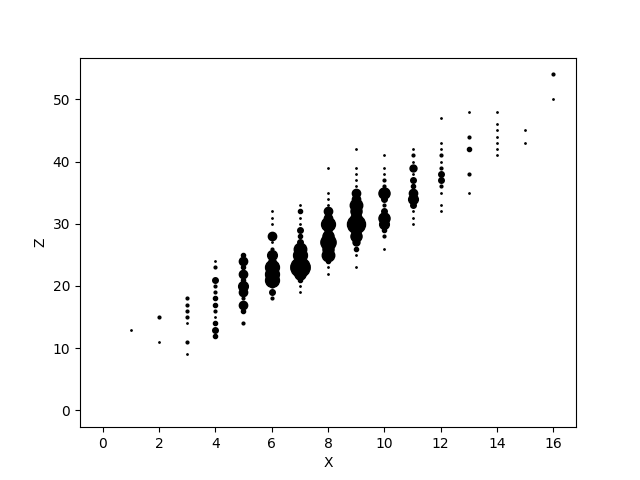
\includegraphics[width=1.1\linewidth]{X_Z_Poiss_Pre}
\end{center}
\vspace*{0\baselineskip}
\end{minipage}
\begin{minipage}{0.333\linewidth}
\begin{center}
	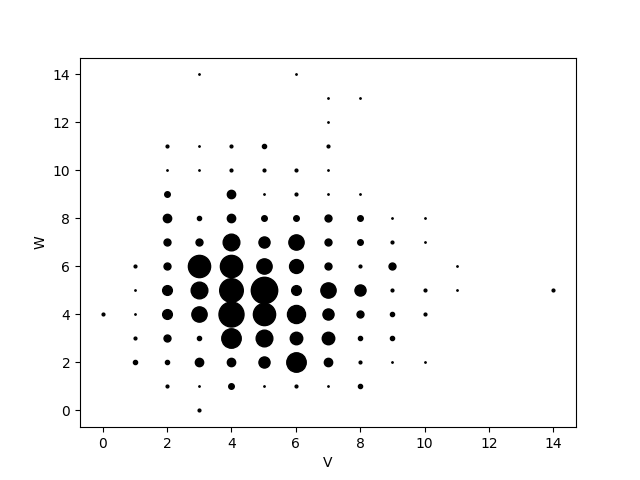
\includegraphics[width=1.1\linewidth]{V_W_Poiss_Pre}
\end{center}
\vspace*{0\baselineskip}
\end{minipage}
\begin{minipage}{0.333\linewidth}
\begin{center}
	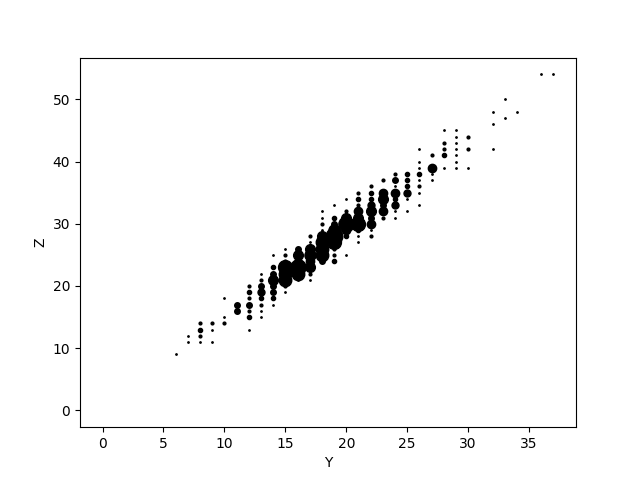
\includegraphics[width=1.1\linewidth]{Y_Z_Poiss_Pre}
\end{center}
\vspace*{0\baselineskip}
\end{minipage}

Wir erkennen, dass $X$ und $Z$, sowie $Y$ und $Z$ stark assoziiert sind. Dies liegt jeweils daran, dass $Z = X + Y + U_Z$ ist und $U_Z \sim \Poiss(1)$ eine relativ kleine Störung ist. Außerdem erkennt man, dass $V$ und $W$ nicht assoziiert sind. Dies liegt daran, dass die exogenen Variablen $U_V$ und $U_W$ als unabhängig angenommen werden.\\

\begin{minipage}{0.5\linewidth}
\begin{center}
\begin{tikzpicture}[->,>=stealth,shorten >=1pt,auto,node distance=2cm,semithick]
  \node (U_X) {$U_X$};
  \node (U_V) [right of=U_X] {$U_V$};
  \node (U_W) [right of=U_V] {$U_W$};
  \node[endo] (X) [below of=U_X] {$X$};
  \node[endo] (V) [below of=U_V] {$V$};
  \node[endo] (W) [below of=U_W] {$W$};
  \node[endo] (Z) [below of=X] {$Z$};
  \node[endo] (Y) [below of=V] {$Y = 3$};
  \node (U_Z) [below of=Z] {$U_Z$};
  \node (U_Y) [below of=Y] {$3$};
  
  \path (U_V) edge node {} (V);
  \path (U_W) edge node {} (W);
  \path (U_X) edge node {} (X);
  \path (U_Y) edge node {} (Y);
  \path (U_Z) edge node {} (Z);
  \path (V) edge node {} (X);
  \path (X) edge node {} (Z);
  \path (Y) edge node {} (Z);
\end{tikzpicture}
\end{center}
\end{minipage}
\begin{minipage}{0.5\linewidth}
Wir führen nun die Intervention $\Do(Y = 3)$ durch. Diese löscht die Pfeile von $V$, $W$ und $X$ zu $Y$, denn $\Pa(Y) = \{ V, W, X \}$. Der modifizierte Kausalgraph ist links abgebildet.\\
Wir würden erwarten, dass das Streudiagramm von $V$ mit $W$ aufgrund der Lokalität unverändert bleibt. Weiter sollte sich der Plot von $X$ mit $Z$ nicht stark verändern, da der Einfluss von $Y$ konstant wird. Außerdem sollte sich das Streudiagramm von $Y$ mit $Z$ zu einer Linie vereinfachen, da $Y$ konstant ist. Die entsprechenden Plots sind darunter abgebildet.\\
\end{minipage}

\begin{minipage}{0.333\linewidth}
\begin{center}
	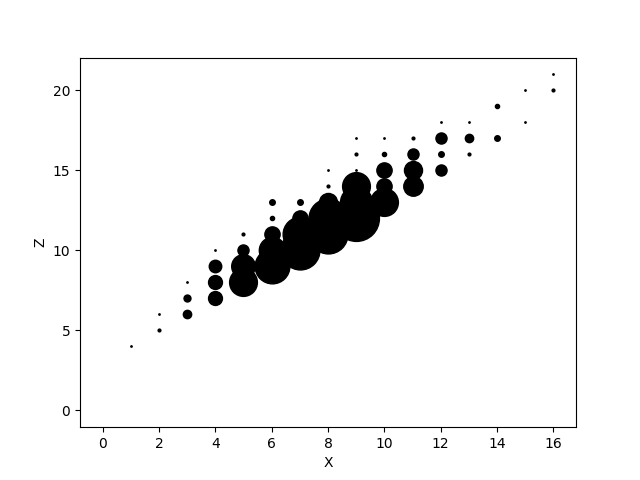
\includegraphics[width=1.1\linewidth]{X_Z_Poiss_Post}
\end{center}
\vspace*{0\baselineskip}
\end{minipage}
\begin{minipage}{0.333\linewidth}
\begin{center}
	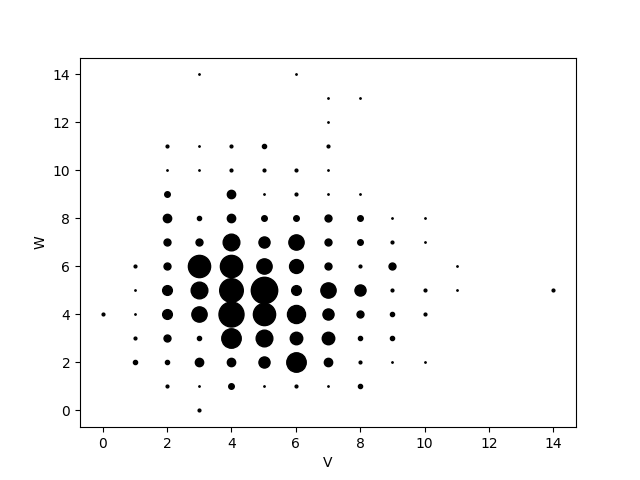
\includegraphics[width=1.1\linewidth]{V_W_Poiss_Post}
\end{center}
\vspace*{0\baselineskip}
\end{minipage}
\begin{minipage}{0.333\linewidth}
\begin{center}
	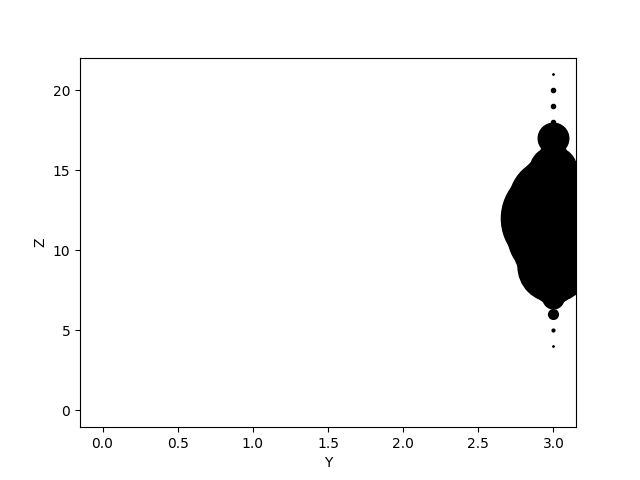
\includegraphics[width=1.1\linewidth]{Y_Z_Poiss_Post}
\end{center}
\vspace*{0\baselineskip}
\end{minipage}

Wir erkennen, dass unsere Vorhersagen tatsächlich eingetroffen sind.\\

Wenn wir nun die Verteilung von $Z$ unter der Intervention von $\Do(Y = 3)$ berechnen wollen, so erhalten wir mit der Regel vom kausalen Effekt für $Z \in \mathbb{N}_0$
\begin{align*}
\mathbb{P}(Z = 10 \mid \Do(Y = 3)) = \sum_{(v, w, x) \in \mathbb{N}_0^3}& \mathbb{P}(Z = 10 \mid Y = 3, V = v, W = w, X = x)\\
&\cdot \mathbb{P}(V = v, W = w, X = x)~.
\end{align*}
Da dies eine abzählbare Summe ist und die bedingten Wahrscheinlichkeiten aufgrund der Abhängigkeiten nicht so einfach berechenbar sind, wurde die folgende Simulation mit $\mathtt{N = 1000000}$ Versuchen durchgeführt.

\begin{lstlisting}
import numpy as np

N = 10**6

V = np.random.poisson(5, N)
X = V + np.random.poisson(3, N)
Y = 3 * np.ones(N, dtype=int)
Z = X + Y + np.random.poisson(1, N)

Wsk = len(np.where(Z == 10)[0]) / N
\end{lstlisting}

$\mathtt{np.where}$ liefert die Indizes der Einträge von $Z$ mit $Z = 10$. Dieser Code liefert
\[\mathbb{P}(Z = 10 \mid \Do(Y = 3)) \approx 12 \%~.\]
Dies stimmt auch mit dem Streudiagramm von oben überein. Dort sehen wir, dass ein nicht unerheblicher Teil der schwarzen Fläche bei $Z = 10$ liegt.
\end{NewBeispiel}

\begin{NewBeispiel}{(Normalverteilung)}
Nun betrachten wir ein Beispiel für eine Intervention bei einem kausalen Modell von normalverteilten Zufallsvariablen.\\

Gegeben seien die folgenden unabhängigen, exogenen Variablen\\
\begin{minipage}{0.5\linewidth}
\begin{align*}
U_V &\sim \mathcal{N}(0, 1)\\
U_W &\sim \mathcal{N}(0, 2)\\
U_X &\sim \mathcal{N}(0, 1)\\ 
U_Y &\sim \mathcal{N}(0, 0.1)\\
U_Z &\sim \mathcal{N}(0, 0.2)~.
\end{align*}
Weiter nehmen wir die folgenden Abhängigkeiten an
\begin{align*}
V &:= U_V\\
W &:= U_W\\
X &:= W + U_X\\
Y &:= W + X + U_Y\\
Z &:= V + Y + U_Z~.
\end{align*}
Dies ergibt den rechts abgebildeten Kausalgraphen.\\
\end{minipage}
\begin{minipage}{0.5\linewidth}
\begin{center}
\begin{tikzpicture}[->,>=stealth,shorten >=1pt,auto,node distance=2cm,semithick]
  \node (U_V) {$U_V$};
  \node (H_eins) [right of=U_V] {};
  \node (U_W) [right of=H_eins] {$U_W$};
  \node[endo] (V) [below of=U_V] {$V$};
  \node[endo] (W) [below of=U_W] {$W$};
  \node[endo] (Z) [below of=V] {$Z$};
  \node (H_zwei) [below of=H_eins] {};
  \node[endo] (Y) [below of=H_zwei] {$Y$};
  \node[endo] (X) [below of=W] {$X$};
  \node (U_Z) [below of=Z] {$U_Z$};
  \node (U_Y) [below of=Y] {$U_Y$};
  \node (U_X) [below of=X] {$U_X$};
  
  \path (U_V) edge node {} (V);
  \path (U_W) edge node {} (W);
  \path (V) edge node {} (Z);
  \path (W) edge node {} (X);
  \path (W) edge node {} (Y);
  \path (Y) edge node {} (Z);
  \path (X) edge node {} (Y);
  \path (U_X) edge node {} (X);
  \path (U_Y) edge node {} (Y);
  \path (U_Z) edge node {} (Z);
\end{tikzpicture}
\end{center}
\end{minipage}

Wir führen nun ein in \textit{in silico Experiment} in R durch. Zur Reproduktion der Ergebnisse kann man $\mathtt{set.seed(31415926)}$ verwenden. Wir lassen $\mathtt{N = 2500}$ Datenpunkte erstellen. Der verwendete Code ist.
\begin{lstlisting}
source("Visualisierung.R")

N = 2500

V = rnorm(N, 0, 1)
W = rnorm(N, 0, 2)
X = W + rnorm(N, 0, 1)
Y = W + X + rnorm(N, 0, 0.1)
Z = V + Y + rnorm(N, 0, 0.2)

Visualisierung(V, W)

Visualisierung(X, Y)

Visualisierung(W, Z)
\end{lstlisting}
$\mathtt{Visualisierung(X, Y)}$ ist eine Funktion die zu $\mathtt{X}$ und $\mathtt{Y}$ den Plot erstellt.
\begin{lstlisting}
library(ggplot2)

Visualisierung = function(X, Y){
  X_name = deparse(substitute(X))
  Y_name = deparse(substitute(Y))
  data = data.frame(X = X, Y = Y)
  ggplot(data, aes(x = X, y = Y)) +
    xlab(X_name) + ylab(Y_name) +
    geom_point(size = 1) + theme_bw() +
    theme(axis.line = element_line(colour = "black"),
          panel.grid.major = element_blank(),
          panel.grid.minor = element_blank(),
          panel.border = element_blank(),
          panel.background = element_blank())
}
\end{lstlisting}

Betrachten wir dieses Experiment nun aus Sicht der Assoziiertheit, so erhalten für die folgenden Plots. Von links nach rechts sind dies die Streudiagramme von $V$ mit $W$, $X$ mit $Y$ und $W$ mit $Z$.\\

\begin{minipage}{0.333\linewidth}
\begin{center}
	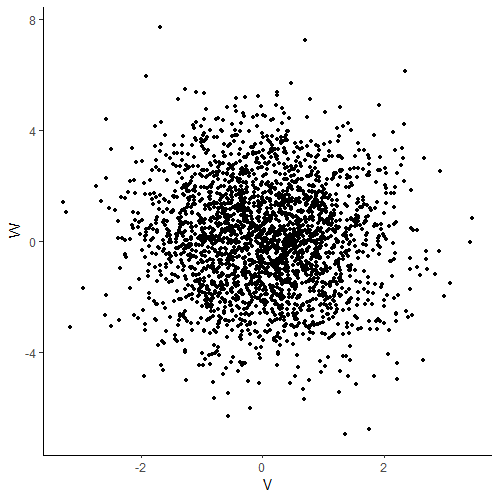
\includegraphics[width=0.9\linewidth]{V_W_Pre.png}
\end{center}
\vspace*{0\baselineskip}
\end{minipage}
\begin{minipage}{0.333\linewidth}
\begin{center}
	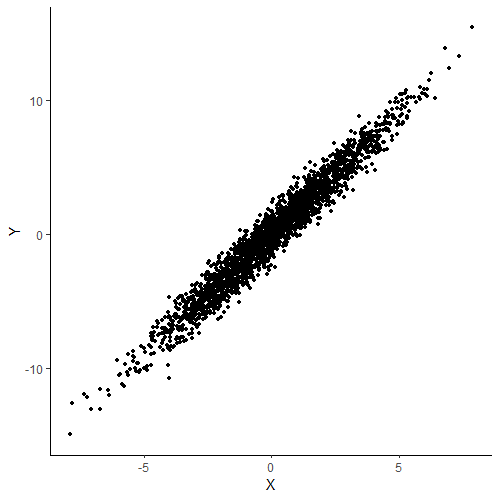
\includegraphics[width=0.9\linewidth]{X_Y_Pre.png}
\end{center}
\vspace*{0\baselineskip}
\end{minipage}
\begin{minipage}{0.333\linewidth}
\begin{center}
	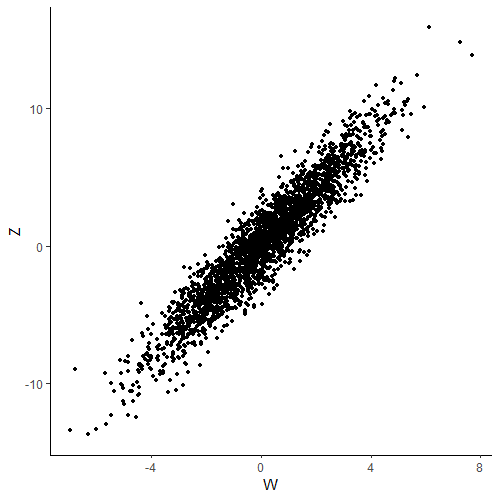
\includegraphics[width=0.9\linewidth]{W_Z_Pre.png}
\end{center}
\vspace*{0\baselineskip}
\end{minipage}

Wir erkennen, dass $V$ und $W$ nicht assoziiert sind. Dies ist auch logisch, da wir $U_V$ und $U_W$ als stochastisch unabhängig angenommen haben. Weiter sind $X$ und $Y$ sehr stark assoziiert. Dies liegt daran, dass $Y := W + X + U_Y$ fast nur durch $X$ bestimmt wird, da $W + U_Y$ als Summe von Normalverteilungen $\mathcal{N}(0, 0.2)$-verteilt ist \cite[S. 59]{MWT}. Dies ist eine kleine Störung, da die Werte aufgrund der geringen Korrelation schwach gestreut sind. Analog sind $W$ und $Z$ stark assoziiert, da $Z := V + Y + U_Z$ stark durch $Y \sim \mathcal{N}(0, 3.1)$ dominiert wird. Hier ist $V + U_Z \sim \mathcal{N}(0, 1.2)$ eine kleine Störung.\\

\begin{minipage}{0.5\linewidth}
\begin{center}
\begin{tikzpicture}[->,>=stealth,shorten >=1pt,auto,node distance=2cm,semithick]
  \node (U_V) {$U_V$};
  \node (H_eins) [right of=U_V] {};
  \node (U_W) [right of=H_eins] {$U_W$};
  \node[endo] (V) [below of=U_V] {$V$};
  \node[endo] (W) [below of=U_W] {$W$};
  \node[endo] (Z) [below of=V] {$Z$};
  \node (H_zwei) [below of=H_eins] {};
  \node[endo] (Y) [below of=H_zwei] {$Y = 2$};
  \node[endo] (X) [below of=W] {$X$};
  \node (U_Z) [below of=Z] {$U_Z$};
  \node (U_Y) [below of=Y] {$2$};
  \node (U_X) [below of=X] {$U_X$};
  
  \path (U_V) edge node {} (V);
  \path (U_W) edge node {} (W);
  \path (V) edge node {} (Z);
  \path (W) edge node {} (X);
  \path (Y) edge node {} (Z);
  \path (U_X) edge node {} (X);
  \path (U_Y) edge node {} (Y);
  \path (U_Z) edge node {} (Z);
\end{tikzpicture}
\end{center}
\end{minipage}
\begin{minipage}{0.5\linewidth}
Wir führen nun die Intervention $\Do(Y = 2)$ durch. Der zugehörige Kausalgraph ist links abgebildet.\\

In R ist der Code für die Intervention $\Do(Y = y)$ der folgende.
\begin{lstlisting}
Intervention_Y = function(y){
  V = rnorm(N, 0, 2)
  W = rnorm(N, 0, 0.1)
  X = W + rnorm(N, 0, 1)
  Y = rep(2, N)
  Z = V + Y + rnorm(N, 0, 0.2)
  data.frame(V = V, W = W, X = X, Y = Y, Z = Z)
}
\end{lstlisting}
\vspace*{0\baselineskip}
\end{minipage}

Die oben betrachteten Streudiagramme sind im modifizierten Modell dann.\\

\begin{minipage}{0.333\linewidth}
\begin{center}
	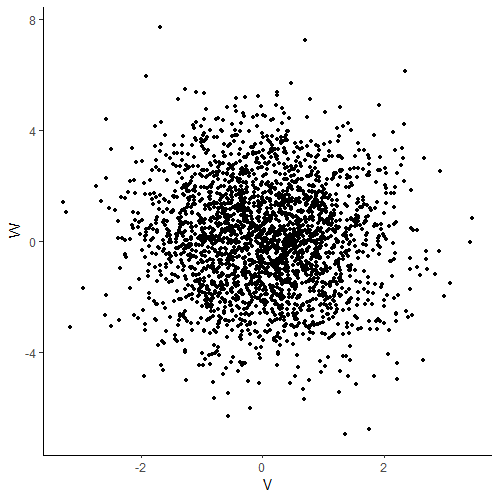
\includegraphics[width=0.9\linewidth]{V_W_Post.png}
\end{center}
\vspace*{0\baselineskip}
\end{minipage}
\begin{minipage}{0.333\linewidth}
\begin{center}
	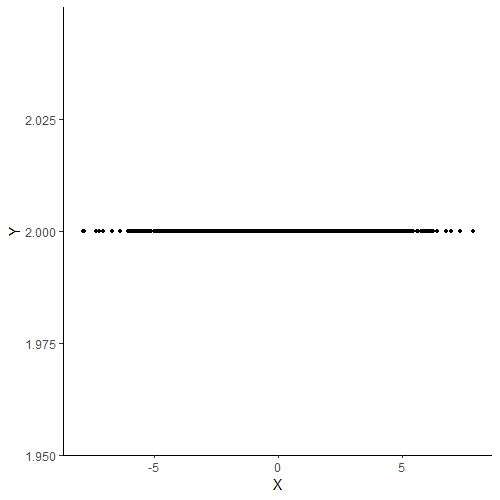
\includegraphics[width=0.9\linewidth]{X_Y_Post.png}
\end{center}
\vspace*{0\baselineskip}
\end{minipage}
\begin{minipage}{0.333\linewidth}
\begin{center}
	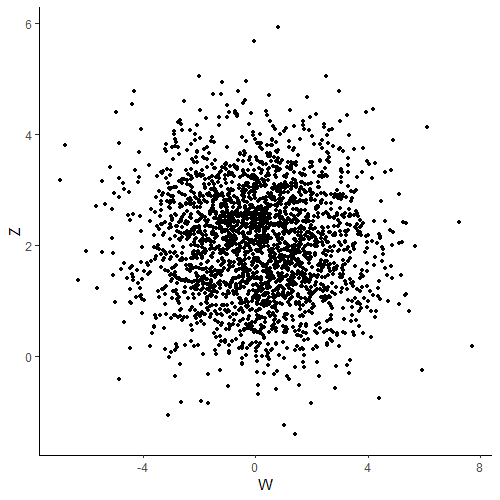
\includegraphics[width=0.9\linewidth]{W_Z_Post.png}
\end{center}
\vspace*{0\baselineskip}
\end{minipage}

Wir erkennen, dass sich der Plot von $V$ und $W$ nicht verändert hat. Dies folgt aufgrund der Lokalität. Weiter scheinen $X$ und $Y$ nun sehr stark assoziiert zu sein. Dies liegt aber daran, dass $Y$ nur den Wert $2$ annimmt. Wir erkennen weiter, dass $W$ und $Z$ nicht mehr assoziiert sind. Durch die Intervention haben wir alle Verbindungslinien von $W$ und $Z$ getrennt.\\

Hier liese sich jetzt die Frage stellen, wie man die Regel vom kausalen Effekt auf stetige Variablen überträgt, um zum Beispiel $\mathbb{P}(Z \in [0, 1] \mid \Do(Y = 2))$ zu berechnen. Wir führen eine Simulation mit $\mathtt{N = 1000000}$ Versuchen durch.

\begin{lstlisting}
N = 10**6
M = 0

for (i in 0:N){
  V = rnorm(1, 0, 1)
  Y = 2
  Z = V + Y + rnorm(1, 0, 0.2)
  if (Z >= 0 && Z <= 1){
    M = M + 1
  }
}

M/N
\end{lstlisting}

Dies liefert
\[\mathbb{P}(Z \in [0, 1] \mid \Do(Y = 2)) \approx 14 \%~.\]
\end{NewBeispiel}

\section{Abgeschnittene Produktregel}
Wir haben mit der Adjustierungsformel einen Weg gefunden, um eine Intervention an einer Variablen, die von einer anderen Variablen beeinflusst wird. Mit der Regel vom kausalen Effekt, haben wir einen Weg gefunden einer Intervention an einer Variablen, die von mehreren Variablen abhängt durchzuführen. Wir können dies nun versuchen weiter zu verallgemeinern zu folgendem

\begin{NewSatz}{(Abgeschnittene Produktregel)\cite[S.60]{Primer}}
Sei ein Kausalgraph gegeben und $X_1, \dots, X_n$ alle Variablen in diesem Modell, sowie $x_1, \dots, x_n$ jeweils Werte dieser Zufallsvariablen. Sei $X$ eine Zufallsvektor mit Variablen aus dem Modell. Ist $x$ ein Wert des Zufallsvaktors, so gilt die \textit{abgeschnittene Produktregel}
\[\mathbb{P}(X_1 = x_1, \dots, X_n = x_n \mid \Do(X = x)) = \prod_{i \in I} \mathbb{P}(X_i = x_i \mid \Pa(X_i) = \pa(X_i))~.\]
Hierbei sei $I \subset \{1, \dots, n\}$ die Menge aller Indizes der Variablen, die nicht in $X$ sind. Weiter sei $x$ und $\pa(X_i)$ konsistent mit $x_1, \dots, x_n$.\\
Ist dies nicht konsistent, so verschwindet die Interventionswahrscheinlichkeit.
\end{NewSatz}

Im ersten Abschnitt tauchte bereits eine ähnliche Formel auf.

\begin{NewSatz}{(Produktdekomposition)\cite[S.29]{Primer}}
Sei ein Kausalgraph gegeben und $X_1, \dots, X_n$ alle Variablen in diesem Modell, sowie $x_1, \dots, x_n$ jeweils Werte dieser Zufallsvariablen. Es gilt die folgende \textit{Produktdekomposition}
\[\mathbb{P}(X_1 = x_1, \dots, X_n = x_n) = \prod_{i=1}^n \mathbb{P}(X_i = x_i \mid \Pa(X_i) = \pa(X_i))~.\]
Hierbei sei $\pa(X_i)$ konsistent mit $x_1, \dots, x_n$.
\end{NewSatz}

\begin{NewBemerkung}{(Produktdekomposition und abgeschnittene Produktregel)}
Durch den Vergleich der Formel für die Produktdekomposition und die abgeschnittenen Produktregel erkennt man, dass diese sehr ähnlich sind.\\
Geht man von der Produktdekomposition aus, so führt die Intervention $\Do(X = x)$ dazu, dass im Produkt alle Faktoren wegfallen, auf die interveniert wird.
\end{NewBemerkung}

Zur Anwendung der abgeschnittenen Produktregel betrachten wir das folgende
\begin{NewBeispiel}{(Poissonverteilung)}
Wir betrachten noch einmal den Kausalgraphen aus dem Poissonverteilungsbeispiel.
\begin{center}
\begin{tikzpicture}[->,>=stealth,shorten >=1pt,auto,node distance=2cm,semithick]
  \node (U_X) {$U_X$};
  \node (U_V) [right of=U_X] {$U_V$};
  \node (U_W) [right of=U_V] {$U_W$};
  \node[endo] (X) [below of=U_X] {$X$};
  \node[endo] (V) [below of=U_V] {$V$};
  \node[endo] (W) [below of=U_W] {$W$};
  \node[endo] (Z) [below of=X] {$Z$};
  \node[endo] (Y) [below of=V] {$Y$};
  \node (U_Z) [below of=Z] {$U_Z$};
  \node (U_Y) [below of=Y] {$U_Y$};
  
  \path (U_V) edge node {} (V);
  \path (U_W) edge node {} (W);
  \path (U_X) edge node {} (X);
  \path (U_Y) edge node {} (Y);
  \path (U_Z) edge node {} (Z);
  \path (V) edge node {} (X);
  \path (V) edge node {} (Y);
  \path (W) edge node {} (Y);
  \path (X) edge node {} (Y);
  \path (X) edge node {} (Z);
  \path (Y) edge node {} (Z);
\end{tikzpicture}
\end{center}

Wir betrachten nun
\begin{align*}
&\mathbb{P}(V = v, W = w, X = x, Y = y, Z = z \mid \Do(V = v, W = w))\\
&= \mathbb{P}(X = x \mid \Pa(X) = \pa(X)) \cdot \mathbb{P}(Y = y \mid \Pa(Y) = \pa(Y)) \cdot \mathbb{P}(Z = z \mid \Pa(Z) = \pa(Z))\\
&= \mathbb{P}(X = x \mid V = v) \cdot \mathbb{P}(Y = y \mid V = v, W = w, X = x) \cdot \mathbb{P}(Z = z \mid X = x, Y = y)~.
\end{align*}
\end{NewBeispiel}

\section{Probleme}
Die Theorie der Interventionen hat einige Probleme \cite[S. 12f]{Paper}.
\begin{enumerate}[label=(\roman*)]
\item Wir haben bei der Definition einer Intervention vorausgesetzt, dass sie lokal ist und somit keine Änderungen an anderen Variablen auftreten. Diese Voraussetzung ist sehr stark und im Allgemeinen nicht erfüllt. Beim Blutdruck und Geschlecht Beispiel haben wir den Blutdruck mithilfe eines Medikaments fixiert. Dies könnte die Heilung mitbeeinflussen.
\item Wie führt man eine Intervention an einer nicht-manipulierbaren Variablen durch. Im Pflanzenbeispiel kann man das Wetter nur bedingte beeinflussen.
\item Die Voraussetzung eines azyklischen Graphen ist stark. In der Realität gibt es viele Beispiel, in der es Rückkopplungen \en{feedback loop} von einer Variablen mit sich selbst gibt. Ein Beispiel ist Inflation und Gehalt. Eine höhere Inflation führt zu mehr Gehalt, was zu einer höheren Inflation führt und so weiter.
\item Die Interpretation des ungerichteten Graphen, der die korrelativen Zusammenhänge zeigt, als einen Kausalgraphen. Dies kann zu Problemen führen, da Korrelation nicht immer Kausalität ist.
\item Eng damit verbunden ist, wie man den Kausalgraphen überhaupt findet. Als Beispiel könnte man sich überlegen, welche Dinge Einfluss auf die Intelligenz haben. Hier gibt es eine sehr große Anzahl an möglichen Variablen, die dies beeinflussen.
\item Wie gut ist das Modell durch die exogenen Variablen beschrieben. Wurden damit genug Informationen eingebaut oder gibt es ungemessene Einflüsse die das kausale Bild verzerren.
\item Ein grundlegendes Problem der Statistik. Wie genau beschreiben die gemessenen Daten die Realität.
\item Wie man die Adjustierungsformel und die Regel vom kausalen Effekt bei stetigen Variablen verwenden kann.
\end{enumerate}
\end{document}

%%% Local Variables:
%%% mode: latex
%%% TeX-master: t
%%% End:
